%&pdflatex
\documentclass[11pt,onecolumn]{scrartcl}
\usepackage[utf8]{inputenc}
\usepackage{amsmath,amssymb,amsfonts,mathrsfs,amsthm}
\usepackage[top=2cm,bottom=3cm,left=2.5cm,right=2cm]{geometry}
\usepackage{amssymb}
\usepackage{amscd}
\usepackage{listings}
\usepackage{array}
\usepackage{mathtools}
\usepackage{dsfont}
\usepackage{graphicx}
\usepackage{pdfpages}
\usepackage[textsize=footnotesize,color=green]{todonotes}
\usepackage{algorithm, algorithmic}
\usepackage{array}
\usepackage{bm}
\usepackage{tikz}
\usepackage{subfigure}
\usepackage[normalem]{ulem}

\newcommand{\bs}[1]{\boldsymbol{#1}}
\DeclareMathOperator{\diag}{diag}

\newcommand{\equaldef}{\stackrel{\mathrm{def}}{=}}

\newcommand{\tablab}[1]{\label{tab:#1}}
\newcommand{\tabref}[1]{Table~\ref{tab:#1}}

\newcommand{\theolab}[1]{\label{theo:#1}}
\newcommand{\theoref}[1]{\ref{theo:#1}}
\newcommand{\eqnlab}[1]{\label{eq:#1}}
\newcommand{\eqnref}[1]{\eqref{eq:#1}}
\newcommand{\seclab}[1]{\label{sec:#1}}
\newcommand{\secref}[1]{\ref{sec:#1}}
\newcommand{\lemlab}[1]{\label{lem:#1}}
\newcommand{\lemref}[1]{\ref{lem:#1}}

\newcommand{\mb}[1]{\mathbf{#1}}
\newcommand{\mbb}[1]{\mathbb{#1}}
\newcommand{\mc}[1]{\mathcal{#1}}
\newcommand{\nor}[1]{\left\| #1 \right\|}
\newcommand{\snor}[1]{\left| #1 \right|}
\newcommand{\LRp}[1]{\left( #1 \right)}
\newcommand{\LRs}[1]{\left[ #1 \right]}
\newcommand{\LRa}[1]{\left\langle #1 \right\rangle}
\newcommand{\LRc}[1]{\left\{ #1 \right\}}
\newcommand{\LRb}[1]{\left| #1 \right|}

\newcommand{\tanbui}[2]{\textcolor{blue}{\sout{#1}} \textcolor{red}{#2}}
\newcommand{\Grad} {\ensuremath{\nabla}}
\newcommand{\Div} {\ensuremath{\nabla\cdot}}
\newcommand{\Nel} {\ensuremath{{N^\text{el}}}}
\newcommand{\jump}[1] {\ensuremath{\LRs{\!\left[#1\right]\!}}}
\newcommand{\uh}{\widehat{u}}
\newcommand{\fnh}{\widehat{f}_n}
\renewcommand{\L}{L^2\LRp{\Omega}}
\newcommand{\pO}{\partial\Omega}
\newcommand{\Gh}{\Gamma_h}
\newcommand{\Gm}{\Gamma_{-}}
\newcommand{\Gp}{\Gamma_{+}}
\newcommand{\Go}{\Gamma_0}
\newcommand{\Oh}{\Omega_h}

\newcommand{\eval}[2][\right]{\relax
  \ifx#1\right\relax \left.\fi#2#1\rvert}

\def\etal{{\it et al.~}}

\newcommand{\vect}[1]{\ensuremath\boldsymbol{#1}}
\newcommand{\tensor}[1]{\underline{\vect{#1}}}
\newcommand{\del}{\Delta}
\newcommand{\grad}{\nabla}
\newcommand{\curl}{\grad \times}
\renewcommand{\div}{\grad \cdot}
\newcommand{\ip}[1]{\left\langle #1 \right\rangle}
\newcommand{\eip}[1]{a\left( #1 \right)}
\newcommand{\pd}[2]{\frac{\partial#1}{\partial#2}}
\newcommand{\pdd}[2]{\frac{\partial^2#1}{\partial#2^2}}

\newcommand{\circone}{\ding{192}}
\newcommand{\circtwo}{\ding{193}}
\newcommand{\circthree}{\ding{194}}
\newcommand{\circfour}{\ding{195}}
\newcommand{\circfive}{\ding{196}}

\def\arr#1#2#3#4{\left[
\begin{array}{cc}
#1 & #2\\
#3 & #4\\
\end{array}
\right]}
\def\vecttwo#1#2{\left[
\begin{array}{c}
#1\\
#2\\
\end{array}
\right]}
\def\vectthree#1#2#3{\left[
\begin{array}{c}
#1\\
#2\\
#3\\
\end{array}
\right]}
\def\vectfour#1#2#3#4{\left[
\begin{array}{c}
#1\\
#2\\
#3\\
#4\\
\end{array}
\right]}

\newtheorem{proposition}{Proposition}
\newtheorem{corollary}{Corollary}
\newtheorem{theorem}{Theorem}
\newtheorem{lemma}{Lemma}

\newcommand{\G} {\Gamma}
\newcommand{\Gin} {\Gamma_{in}}
\newcommand{\Gout} {\Gamma_{out}}

\newtheorem{remark}{Remark}

\author{Jesse Chan\textsuperscript{a}, Jay Gopalakrishnan\textsuperscript{b}, and Leszek Demkowicz\textsuperscript{a}}

%\title{$\epsilon$-explicit analysis of DPG for convection-dominated diffusion}
\title{Global properties of DPG test spaces for convection-diffusion problems}
\date{}
\begin{document}

\maketitle
\begin{center}
\textsuperscript{a} Institute for Computational Engineering and Sciences, \\University of Texas at Austin, \\Austin, TX 78712, USA\\
\end{center}

\begin{center}
\textsuperscript{b} Department of Mathematics\\Portland State University, \\
Portland, OR 97207, USA
%\textsuperscript{b} Facultad de Matem\'aticas, \\Pontificia Universidad Cat\'olica de Chile,\\
%Avenida Vicu\~na Mackenna 4860, Santiago, Chile
\end{center}

%\tableofcontents

\section{Introduction to DPG}

The Discontinuous Petrov-Galerkin method was originally introduced by Demkowicz and Gopalakrishnan in 2009 as a way to attain automatic inf-sup stability for any well-posed variational problem through the construction of optimal test functions \cite{DPG2}.  The method was later shown to be equivalent to the minimum residual method applied to the operator residual corresponding to a variational formulation \cite{DPG2, ChanHeuerBui-ThanhDemkowicz12}.  A more detailed overview of the current state of DPG is available at \cite{overviewDPG}; we give only a brief introduction here.

The derivation of the DPG method can be briefly summarized as follows: assume we are given a trial space $U$, a discrete trial space $U_h \subset U$, a Hilbert test space $V$, and a well-posed (in the inf-sup sense) variational problem: find $u\in U$  such that
\begin{align}
\label{variational}
&b(u,v) = l(v), \quad \forall v\in V, 
\end{align}
where $b(u,v)$ is a bilinear form and $l \in V'$. If we identify the variational operator $B: U\rightarrow V'$ such that $\LRa{Bu,v} \coloneqq b(u,v)$, we can write the above variational formulation as an operator equation in $V'$
\[
Bu = l,
\]
where inf-sup well-posedness of the variational formulation translates to boundedness from above and below of the operator $B$.  

Let $u_h \in U_h$ now be a discrete approximation to $u$. Seeking the minimization of the discrete residual $\frac{1}{2} \nor{Bu_h-l}^2_{V'}$, we arrive at the normal equations 
\begin{equation}
\label{dualNormal}
\LRp{Bu_h-l,B\delta u}_{V'} = 0, \quad \forall \delta u \in U_h.  
\end{equation}
Since $V$ is Hilbert, we can introduce the Riesz map $R_V:V \rightarrow V'$, an isometric isomorphism such that $\LRa{R_V v,\cdot} = \LRp{v,\cdot}_V$. By taking the inverse of the Riesz map, we can transform the normal equations in $V'$ to a set of normal equations in $V$
\[
\LRp{R_V^{-1}\LRp{Bu_h-l},R_V^{-1}\LRp{B\delta u}}_{V} = 0, \quad \forall \delta u \in U_h.  
\]
Using the definitions of the Riesz map $R_V$ and variational operator $B$, we have that
\begin{align*}
\LRp{R_V^{-1}\LRp{Bu_h-l},R_V^{-1}\LRp{B\delta u}}_{V} = 0, \quad \forall \delta u \in U_h \\
\rightarrow \LRa{Bu_h-l,R_V^{-1}\LRp{B\delta u}}_{V} = 0, \quad \forall \delta u \in U_h \\
\rightarrow b\LRp{u_h,R_V^{-1} B\delta u} - l\LRp{R_V^{-1} B\delta u} = 0, \quad \forall \delta u \in U_h.
\end{align*}
In other words, the minimization of the operator residual associated with a given variational form corresponds directly to a Petrov-Galerkin formulation, where test functions are determined under the so-called \textit{trial-to-test} operator $R_V^{-1}B$, which, given functions in the discrete trial space $U_h$,  returns back corresponding test functions which span the discrete test space.  

Solutions $u$ to the above problem enjoy the following properties: 
\begin{enumerate}
\item If we define the energy norm 
\[
\nor{u}_E = \nor{Bu}_{V'} = \sup_{v\in V\setminus\{0\}}\frac{\LRb{b(u,v)}}{\nor{v}_V},
\]
then DPG is optimal in the energy norm $\nor{u}_E$, which is induced through the energy inner product
\[
\LRp{v,w}_E = \LRp{Bv,Bw}_{V'} = \LRp{R_V^{-1}Bv, R_V^{-1}Bw}_V.
\]
\item The exact energy error $\nor{u-u_h}_E$ is computable without knowing $u$ explicitly, owing to the fact that
\[
\nor{u-u_h}_E = \nor{B(u-u_h)}_{V'} = \nor{{l-Bu_h}}_{V'} = \sup_{v\in V\setminus\{0\}}\frac{l(v)-b(u,v)}{\nor{v}_V},
\]
which can be computed by first computing an \textit{error representation function} $e$ and then evaluating $\nor{e}_V$.  The error representation function is determined by solving the problem
\[
\LRp{e,\delta v}_V = l(\delta v)-b(u,\delta v), \quad \delta v\in V.
\]
This property is simply a result of the minimum residual nature of DPG; the energy error is simply the residual, measured in the proper norm.  
\item Let $\{u_i\}_{i = 0}^{i = N}$ be discrete trial functions and $v_{u_i}$ be the corresponding optimal test functions (solutions of Problem (\ref{aux}) below).  The discrete system resulting from DPG is symmetric positive-definite; this can be seen from the identity
\[
b(u_i,v_{u_j}) = \LRp{v_{u_i},v_{u_j}}_V = \LRp{v_{u_j},v_{u_i}}_V = b(u_j,v_{u_i}).
\]
Positive-definiteness is again a natural consequence of the minimum-residual nature of DPG.  
\end{enumerate}

\subsection{Broken test spaces}

To determine test functions under DPG, we must invert the Riesz map by determining $R_V^{-1} B\delta u$, which is done by solving the auxiliary variational problem
\begin{equation}
\label{aux}
(v,\delta v)_V = b\LRp{\delta u,\delta v}, \quad \forall \delta v\in V.  
\end{equation}
Unfortunately, this amounts to both an infinite-dimensional and global problem if $V$ is not chosen carefully.  For example, if $V = H^1(\Omega)$ and $\LRp{\cdot, \cdot }_V$ corresponded to the $H^1$ Sobolev inner product  $\LRp{v,\delta v}_{L^2(\Omega)} + \LRp{\grad v,\grad \delta v}_{L^2(\Omega)}$, solving for a single optimal test function would be equivalent to solving the Poisson equation exactly over the entire domain.  However, we can both localize and make solving Problem~(\ref{aux}) computationally feasible by choosing for $V$ a \textit{broken} test space and by approximating the solution to (\ref{aux}) using a discrete space $V_h\subset V$.

We begin by assuming we are given some triangulation $\Omega_h$ of $\Omega$ such that $\bar{\Omega} = \bigcup_{K\in \Omega_h}\bar{K}$.  We can adopt for $V$ the broken test space
\[
V(\Oh) = \bigoplus_{K\in \Omega_h}V(K).
\]
If we further assume that the inner product and norm on $V$ are localizable\footnote{A localizable norm $\nor{v}_{V(\Oh)}$ can be written in the form 
$$\nor{v}_{V(\Oh)}^2 = \sum_{K\in\Oh} \nor{v}_{V(K)}^2,$$ where $\nor{v}_{V(K)}$ is a norm over the element $K$.}, the solution to \eqref{aux} (corresponding to the inversion of the Riesz map) can now be determined locally over each element.  In practice, these solutions are approximated by solving (\ref{aux}) over a locally conforming space $V_h$ over each element $K$, where $\dim(V_h) > \dim(U_h)$ elementwise.  Typically, if $U_h$ is of order $p$, $V_h$ is chosen to be the corresponding $H^1$ or $H({\rm div})$ conforming space of order $p + \del p$, where $\del p \geq n$, the spatial dimension \cite{practicalDPG}.  For this reason, we refer to $V_h$ as the \textit{enriched} space.  We refer to this approximated test space under $V_h$ as the approximate optimal test space $V_{{\rm opt},h}$.  
\begin{remark}
All properties of DPG carry over if $V=V_h$, the discrete inner product space, and if Problem~(\ref{aux}) is well-approximated under $V_h$, then the solution to our variational problem (\ref{variational}) over the approximate optimal test space will deliver very similar results to the solution of (\ref{variational}) over the exact optimal test space.  
\end{remark}

\subsection{The ultra-weak variational formulation}

Up to now, the variational formulation has been left unspecified.  For several reasons, we've chosen to use the \textit{ultra-weak formulation}, which results from writing the PDE as a first-order system, integrating all derivatives by parts, and identifying boundary traces as independent unknowns, similarly to hybridized DG methods.  The formulation is given as follows: let $$\Gh = \bigcup_{K\in \Oh} \partial K$$ be the \textit{mesh skeleton}, comprising of the union of all element boundaries.  Let $Au=f$ represents the strong form of a first-order system of PDEs; the ultra-weak formulation is then
\begin{equation}
\label{variationalProblem}
b\LRp{\LRp{u,\uh},v} = \LRp{u,A_h^*v}_{\Oh} + \sum_{K \in \Oh} \LRa{\uh,v}_{\partial K} = \LRp{f,v}_{\Omega},
\end{equation}
where $u \in \L$, and $A_h^*$ is the formal adjoint of $A$ acting elementwise on a broken test space, and $\LRa{\uh,v}_{\partial K}$ is the duality pairing between the trace unknown $\uh$ and the trace of the test function $v$ on an element boundary.  Under proper regularity assumptions, we have that 
$$\sum_{K \in \Oh} \LRa{\uh,v}_{\partial K} = \LRa{\uh,\jump{v}}_{\Gh}.$$    %so $\uh \in \gamma(D\LRp{A})$, the trace space of the domain of the strong operator $A$.  
Finally, $\uh$ represents the trace of the conforming solution to $Au=f$ on the mesh skeleton $\Gh$; if we define the graph space $H_A \coloneqq \LRc{u \in U: Au\in \L},$ then $\uh$ comes from $ \widehat{H}_A(\Gh)$, the trace space of $H_A$ on $\Gh$
\[
\widehat{H}_A(\Gh) \coloneqq \LRc{ \left.u\right|_{\Gh}: u\in H_A}.
\]

Combining this variational formulation with the concept of DPG optimal test functions yields a conforming method for $u$, the field variable, and $\uh$, the trace variable. Optimal test functions are all determined locally, and optimal test functions corresponding to traces defined on the element boundary $\partial K$ have support over each element adjacent to $\partial K$.  The degrees of freedom are thus coupled together globally through the optimal test functions for trace variables.  

\begin{remark}
\label{remarkDahmen}
It is possible to apply the same minimum-residual method behind DPG in an alternative fashion by casting the normal equations as a saddle-point problem, which is the approach taken by Dahmen et al.\ in \cite{DahmenVariationalStabilization}. This method requires the solution of a larger global linear system than the DPG method, but can be directly applied to arbitrary variational formulations and conforming discretizations of $V$.  
\end{remark}

\subsection{The graph test norm}

We have not yet specified the inner product $\LRp{v,\delta v}_V$, which induces the norm defining the space $V$.  Here, we derive two important ``canonical" test norms for the ultra-weak variational formulation.  We begin first with the canonical norm in $U$. Since $\uh \in \widehat{H}_A(\Gh)$, the standard norm for $\uh$ is the so-called minimum energy extension norm defined as
\begin{equation*}
\|\widehat{u}\| = \inf_{w\in \widehat{H}_A(\Gamma_h),
  \left.w\right|_{\Gh}=\widehat{u}} \|w\|_{\widehat{H}_A}.
\end{equation*}
The canonical norm for the group variable $\LRp{u,\uh}$ is then given by
\[
\|\left(u,\widehat{u}\right)\|_U^2 = \|u\|^2_{\L} + \|\widehat{u}\|^2.
\]
If we define the norm $\nor{v}_{V,U}$  through
\[
\nor{v}_{V,U}^2 = \|A_h^*v\|_{\L}^2
+\left(\sup_{\widehat{u} \in \widehat{H}_A(\Gamma_h)} \frac{\LRa{ \widehat{u},
  \jump{v} }_{\Gh}}{\|\widehat{u}\|}\right)^2, 
\]
it has been shown in \cite{Bui-ThanhDemkowiczGhattas11a, ChanHeuerBui-ThanhDemkowicz12} that the canonical norm $\nor{\LRp{u,\uh}}_U$ in $U$ induces (generates) the norm $\nor{v}_{V,U}$ in $V$; in other words, the energy norm in which DPG is optimal is equal to the canonical norm $\nor{\LRp{u,\uh}}_U$ if we choose for a test norm on $\nor{v}_{V,U}$.  

The canonical norm $\nor{\LRp{u,\uh}}_U$ in $U$ provides an optimal balance between the standard norms on the field $u$ and the flux $\uh$ \cite{DPG4}. As a result, if the induced norm $\nor{v}_{V,U}$ (namely, the optimal test norm) is used to compute optimal test functions in (\ref{aux}), the finite element error in the canonical norm is the best in the norm $\nor{u}_{U}$. Unfortunately, the optimal test norm is non-localizable due to the presence of the jump term $\jump{v}$. Since the jump terms couple elements together, the evaluation of the jump terms requires contributions from all the elements in the mesh. 
Consequently, solving for an optimal test function amounts to inverting the Riesz map over the entire mesh $\Oh$, making the optimal test norm impractical.

On the other hand, since $A^*_h v \in \L$, we can use as a test norm for $v$ the broken graph test norm: 
\[
\nor{v}_V^2 =  \|A_h^*v\|_{\L}^2 + \nor{v}_{\L}^2,
\]
where we have regularized the seminorm $\nor{A_h^*v}_{\L}^2$ by adding to it the $L^2$ norm of $v$.  

The norm $\nor{v}_V$ can be considered as a localization of $\nor{v}_{V,U}$ to allow for the solution of optimal test functions on an element-by-element basis, and can be considered to be the canonical norm on $V$.  In the DPG literature \cite{DPG4}, $\nor{v}_{V,U}$ is known as the {\em optimal test norm}, while $\nor{v}_{V}$ is known as the quasi-optimal or {\em graph} test norm.  The DPG method was first shown to be well-posed under the graph test norm for the Poisson and convection-diffusion equations in \cite{analysisDPG}.  This analysis was later extended to the large class of Friedrichs' systems in \cite{Bui-ThanhDemkowiczGhattas11b} and to Stokes in \cite{stokesDPG}.  

It has also been shown in \cite{stokesDPG} that $\nor{v}_{V,U}$ and $\nor{v}_V$ are equivalent norms; if the operator $A$ is bounded below such that $\nor{Au}_{\L} \geq \gamma\nor{v}_{\L}$, then the equivalence constants between $\nor{v}_{V,U}$ and $\nor{v}_V$ are $O(\gamma)$.  This is important in context of \textit{singular perturbation problems}, which typically depend on some parameter $k\rightarrow 0$ or $k\rightarrow \infty$; if the constant $\gamma$ associated with the problem is independent of $k$, then the DPG method under the graph test norm is \textit{robust}, or equivalent to the $\L$-projection with constants independent of $k$.  Robustness is discussed more in Section~\ref{sec:robust} in context of the convection-diffusion equation.

\section{The ultra-weak formulation and globally conforming test spaces}

Though DPG test functions are determined locally on an element-by-element basis, it is the global properties of the test space that determine the performance of the method.  We motivate this statement first by deriving global conditions for the test space under which the ultra-weak variational formulation recovers an $L^2$ optimal solution, using the specific example of the convection-diffusion equation.  

\subsection{The convection-diffusion equation}

The convection-diffusion problem models the concentration $u$ of some solvent in a convection field $\beta$ subject to diffusion of some magnitude $\epsilon > 0$ in some domain $\Omega$ with boundary $\Gamma$.  We decompose the boundary as follows:
\begin{align*}
\Gamma_{\rm in} &\coloneqq \{x\in \Gamma; \beta_n(x) < 0\}, \quad {\rm
(inflow)}\\ 
\Gamma_{\rm out} &\coloneqq \{x\in \Gamma; \beta_n(x) > 0\},
\quad {\rm (outflow)}\\
\Gamma_{0} &\coloneqq \{x\in \Gamma;\beta_n(x) = 0\},
\end{align*}
where $\beta_n \coloneqq \beta \cdot n$.

The problem is typically written in as
\begin{align*}
\div\LRp{\beta u - \epsilon \grad u} &= f, \quad \text{in } \Omega \\
u &= u_{0}, \quad \text{on } \Gamma.
\end{align*}
The problem is especially of interest as a prototypical problem for boundary layer problems in computational fluid dynamics, as solutions to the convection-diffusion problem can, for certain boundary conditions, develop strong boundary layers of width $\epsilon$ at the outflow boundary $\Gamma_{\rm out}$.    

We can further write it as a system of first-order equations
\begin{align*}
\div\LRp{\beta u - \sigma} &= f\\
\frac{1}{\epsilon}\sigma - \grad u &= 0.
\end{align*}
This first order system is the starting point for the ultra-weak variational formulation, which, under the convection-diffusion equation and prior to the application of boundary data, is given as 
\begin{align*}
b\LRp{\LRp{u,\sigma, \uh, \fnh}, \LRp{v,\tau}} &=\LRa{\uh,\tau_n}_{\Gh} + \LRa{\fnh,v}_{\Gh} + \\ & \LRp{u, \Grad_h\cdot \tau - \beta\cdot \Grad_h v}_{\L} + \LRp{\sigma, \frac{1}{\epsilon}\tau + \Grad_h v}_{\L}.
\end{align*}
where $\fnh \coloneqq \beta_n u - \sigma_n$.  Trial and test spaces are specified to be 
\begin{align*}
\LRp{u,\sigma} \in \L, \fnh \in H^{-1/2}(\Gh), \uh \in H^{1/2}(\Gh)&,\\ 
v \in H^1(\Oh), \tau \in H\LRp{\rm div, \Oh}&,
\end{align*}
where $H^1(\Oh)$ and $H\LRp{\rm div, \Oh}$ represent the broken $H^1$ and $H(\rm div)$ spaces over $\Oh$.  This is discussed in more detail for the convection-diffusion equation in \cite{DPGrobustness, ChanHeuerBui-ThanhDemkowicz12}.

For the case of boundary data $\uh = u_0$ on the entire boundary $\Gamma$, our variational formulation becomes
\begin{align*}
\LRa{\uh,\tau_n}_{\Gh^0} + \LRa{\fnh,v}_{\Gh} + \LRp{u, \Grad_h\cdot \tau - \beta\cdot \Grad_h v} + \LRp{\sigma, \frac{1}{\epsilon}\tau + \Grad_h v} = \LRp{f,v} + \LRa{u_0,\tau_n}_{\Gamma}, 
\end{align*}
where $\Gh^0 = \Gh\setminus \Gamma$ is the union of all internal element edges, and is referred to as the internal skeleton, and $\Grad_h$ and $\Grad_h\cdot$ are understood to be the broken gradient and divergence, taken over each individual element.  We have also dropped the subscript for $\LRp{\cdot,\cdot}_{L^2(\Omega)}$ and, for the rest of the paper, simply refer to the $L^2$ inner product using the notation $\LRp{\cdot,\cdot}$.  

For DPG, we must also specify a test norm which defines the test space.  Our focus will be on the graph test norm for convection-diffusion, which, under the ultra-weak variational formulation, 
\[
\nor{v}_{V_{\rm graph}}^2 = \nor{\grad_h\cdot\tau - \beta \cdot \grad_h v}_{L^2(\Omega)}^2 + \nor{{\epsilon}^{-1} \tau -  \grad_h v}_{L^2(\Omega)}^2 + \nor{v}_{L^2(\Omega)}^2
\]
where $\grad_h$ and $\div_h$ are understood to act elementwise.\footnote{Since $\nor{A^*_hv}$ is not positive definite on its own, we typically add an $L^2$ term for all components of the test function; however, here the $L^2$ norm of $\tau$ is neglected as it is not required to preserve positive-definiteness of the norm.}

Though our focus is on the convection-diffusion equation, we will attempt to relate concepts to a more general framework and notation when possible.  Overloading the notation $\uh \coloneqq \LRp{\uh,\fnh}$, $u \coloneqq \LRp{u,\sigma}$, and $v \coloneqq \LRp{v,\tau}$, we can define the operator $A_h^*: V(\Oh)\rightarrow \L$ through its action restricted to an individual element $K$
\[
\left.A_h^*v\right|_K = \LRp{\div\tau - \beta \cdot \grad v, {\epsilon}^{-1} \tau -  \grad v}, \quad \text{on } K \in \Oh.
\]
We then have the abstract representation of both the ultra-weak variational formulation and the graph test norm as
\begin{align*}
b\LRp{\LRp{u,\uh},v} &\coloneqq \LRa{\uh,v} + \LRp{u,A^*_h v}_{\L} \\
\nor{v}_V^2 &\coloneqq \nor{A_h^*v}_{\L}^2 + \nor{v}_{\L}^2
\end{align*}
From this point onward, we will continue to overload our abstract notation in order to connect more general concepts with the concrete example of the convection-diffusion equation.

\subsection{$L^2$ optimality under the ultra-weak variational formulation}
We will aim now to define energy settings and test/trial spaces under which the ultra-weak formulation produces $L^2$-optimal solutions for $u,\sigma$.  Our approach focuses on the convection-diffusion equation, but we will generalize using more abstract notation when possible.  

\subsubsection{Test and trial spaces}
We begin by defining the spaces
\begin{align*}
H_A &= \LRc{\LRp{u, \sigma} \in H^1(\Omega) \times H({\rm div};\Omega): \LRp{\div\LRp{\beta u - \sigma}, \frac{1}{\epsilon}\sigma - \grad u}  \in L^2\LRp{\Omega}}\\
H_{A^*} &= \LRc{\LRp{v,\tau} \in H^1(\Omega)\times H({\rm div};\Omega): \LRp{\div \tau - \beta\cdot \Grad v, \frac{1}{\epsilon}\tau + \Grad v} \in L^2\LRp{\Omega}}
\end{align*}
Note that in these definitions, we have chosen both trial and test functions from the fully conforming spaces $H({\rm div};\Omega)$ and $H^1(\Omega)$ over $\Omega$.  Let us define the spaces ${U} = {V} = H^1(\Omega) \times H({\rm div};\Omega)$ as the \textit{conforming} spaces for which the inter-element jumps $\LRa{\uh,\tau_n}_{\Gh^0}$ and $\LRa{\fnh,v}_{\Gh^0}$ both vanish.  If we again overload notation by defining ${u} \coloneqq \LRp{u,\sigma}^T\in {U}$ and ${v} \coloneqq \LRp{v,\tau} \in {V}$, and define the operator $A$ and its adjoint $A^*$ through
\[
A{u} \coloneqq \vecttwo{\div\LRp{\beta u - \sigma}}{\frac{1}{\epsilon}\sigma - \grad u}, \quad A^*{v} \coloneqq \vecttwo{\div \tau - \beta\cdot \Grad v}{\frac{1}{\epsilon}\tau + \Grad v},
\]
then we can recognize $H_A$ and $H_{A^*}$ as the \textit{graph spaces} corresponding to the first-order system operator $A$ and its adjoint $A^*$. We can now compactly characterize the spaces $H_A$ and $H_{A^*}$
\[
H_A = \LRc{{u} \in {U}, A{u} \in L^2\LRp{\Omega}}, \quad H_{A^*} = \LRc{{v} \in  {V}, A^*{v} \in L^2\LRp{\Omega}}.
\]
%Under the ultra-weak formulation, we are free to choose $\LRp{u,\sigma} \in L^2(\Omega)$.  
By choosing $\LRp{v,\tau}\in H_{A^*}$, we can eliminate the inter-element jumps in the ultra-weak variational formulation, such that we are left with
\begin{align*}
\LRa{\fnh,v}_{\Gamma} - \LRa{\uh,\tau_n}_{\Gamma} + \LRp{u, \Grad\cdot \tau - \beta\cdot \Grad v} + \LRp{\sigma, \frac{1}{\epsilon}\tau + \Grad v} = \LRp{f,v}
\end{align*}
prior to the application of boundary conditions.  

Specifying spaces for the trace variables $\fnh$ and $\uh$ is a bit more involved.  Note that $H_{A}$ and $H_{A^*}$ are dual to each other; denoting the trace space of $H_A$ as $\widehat{H}_A = H^{1/2}(\Gamma) \times H^{-1/2}(\Gamma)$ and defining the traces (again overloading notation) through $\widehat{v} \coloneqq \LRp{\left.v\right|_\Gamma, \left.\tau_n\right|_\Gamma} = \LRp{\widehat{v},\widehat{\tau}}$, $\widehat{u} \coloneqq \LRp{\fnh,\uh} \in \widehat{H}_A$, we are able to characterize the duality pairing over $\Gamma$ as follows: we have
\[
\LRa{\fnh,v} + \LRa{\uh,\tau_n} \coloneqq \LRp{\div\LRp{\beta u - \sigma},v} + \LRp{\frac{1}{\epsilon}\sigma - \grad u,\tau} - \LRp{u, \Grad\cdot \tau - \beta\cdot \Grad v} - \LRp{\sigma, \frac{1}{\epsilon}\tau + \Grad v}
\]
or, using abstract operator notation
\[
\LRa{\widehat{u},\widehat{{v}}} = (A{u},{v})-({u},A^*{v}).
\]
An interpretation of the above characterization would be that the trial variables $\fnh$ and $\uh$ represent traces of functions $\LRp{\beta u - \sigma, u} \in H_A$.  Our trial and test spaces can now be specified
\[
\LRp{u,\sigma}\in L^2(\Omega), \LRp{\uh,\fnh}\in H^{1/2}(\Gamma) \times H^{-1/2}(\Gamma), \LRp{v,\tau}\in H_{A^*}
\]
or under our more general notation,
\[
u\in L^2(\Omega), \widehat{u}\in \widehat{H}_{A}(\Gamma), v\in H_{A^*}
\]
where $\widehat{H}_{A}(\Gamma) = \LRc{\left.u\right|_\Gamma, u\in H_A}$ consists of the boundary traces of functions in $H_A$.  
Thus, while we formally relax regularity constraints on $\LRp{u,\sigma}$ by simply requiring $\LRp{u,\sigma} \in L^2(\Omega)$, we maintain regularity constraints through our choice of spaces for the trace variables.  

\subsubsection{Test space boundary conditions}
\label{L2OptTestBC}
Having replaced the ultra-weak formulation under a broken test space with the ultra-weak formulation using a globally conforming test space, we now aim to treat boundary conditions.  Under our model problem, boundary data $u_0$ is applied to $\uh$ on the entirety of $\Gamma$, such that our variational formulation becomes
\[
\LRa{\fnh,v}_{\Gamma} + \LRp{u, \Grad\cdot \tau - \beta\cdot \Grad v} + \LRp{\sigma, \frac{1}{\epsilon}\tau + \Grad v} = \LRp{f,v} + \LRa{u_0,\tau_n}_{\Gamma}.
\]
We can restrict our test space\footnote{Formally speaking, we require only that $\LRa{\fnh,v}_\Gamma = 0, \forall \fnh\in H^{-1/2}(\Gamma)$.  However, since $\left.v\right|_\Gamma \in H^{1/2}(\Gamma)$, and since the duality pairing $\LRa{\cdot,\cdot}_{H^{-1/2}(\Gamma)\times H^{1/2}(\Gamma)}$ is definite, this condition is equivalent to $\left.v\right|_\Gamma = 0$.} to $\tilde{H}_{A^*} \coloneqq \LRc{\LRp{v,\tau} \in H_{A^*}, \left.v\right|_\Gamma = 0} \subset H_{A^*}$, which reduces the formulation to
\begin{align*}
\LRp{u, \Grad\cdot \tau - \beta\cdot \Grad v} + \LRp{\sigma, \frac{1}{\epsilon}\tau + \Grad v} &= \LRp{f,v} + \LRa{u_0,\tau_n}_{\Gamma}.
\end{align*}
If our trial space is now taken to be the discrete trial space ${U}_h$ spanned by trial functions $\phi_i = 1,\ldots,N$, by choosing our discrete test space such that 
\begin{align*}
\div \tau - \beta\cdot \Grad v &= u_i\\
\frac{1}{\epsilon}\tau + \Grad v &= \sigma_i\\
v &= 0, \quad \text{on } \Gamma,
\end{align*}
where $u_i$ and $\sigma_i$ are the $u$ and $\sigma$ components of the $i$th trial function $\phi_i$, then our discrete variational problem for $\LRp{u_h,\sigma_h}$ becomes
\begin{align*}
\LRp{u_h,u_i} + \LRp{\sigma_h,\sigma_i}  &= \LRp{u_h, \Grad\cdot \tau - \beta\cdot \Grad v} + \LRp{\sigma_h, \frac{1}{\epsilon}\tau + \Grad v}  \\
&= \LRp{f,v} + \LRa{u_0,\tau_n}_{\Gamma} \\
&= \LRp{u,u_i} + \LRp{\sigma,\sigma_i}
\end{align*}
and the solutions $u_h,\sigma_h \in {U}_h$ to our discrete variational problem are exactly the best $L^2$-approximations to the $u$ and $\sigma$.

We can frame the above discussion concerning boundary conditions using a more abstract notation as well; let us define an boundary condition operator $C:\widehat{H}_{A} \rightarrow \widehat{H}_{A}$, such that boundary data is applied to the quantity $\LRa{C\widehat{u},\widehat{v}}$.  For the convection-diffusion equation, $C\widehat{u} = \LRp{\uh,0}$, and $\LRa{C\widehat{u},\widehat{v}} \coloneqq \LRa{\uh,\tau_n}$.  Due to the definiteness of the duality pairing $\LRa{\cdot,\cdot}$, we have that $\LRa{C\widehat{u},\widehat{v}} = \LRa{\widehat{u},C'\widehat{v}}$, where $C'$ is the conjugate of $C$ with respect to the duality pairing.  Next, we define the space $\tilde{H}_{A^*}$ as
\[
\tilde{H}_{A^*} = \LRc{v\in H_{A^*}, (I-C')\widehat{v} = 0}.
\]
We interpret $\tilde{H}_{A^*}$ as being the subspace of $H_{A^*}$, the graph space of conforming test functions, such that the remaining boundary terms vanish after imposition of boundary data.  

\begin{remark}
For non-homogeneous boundary conditions under standard finite element methods, boundary conditions are treated using lift and extension operators.  In other words, given boundary data $u_0$ on some part of the boundary $\Gamma_0 \subset \Gamma$, then we decompose our solution $u$ into $u = E u_0 + \tilde{u}$, where $\tilde{u}$ comes from a so-called homogeneous space $\tilde{{U}} \coloneqq {U}/Eu_0$, and $Eu_0$ is a non-unique extension of the lift $u_0$ into the interior of the domain $\Omega$.  Under a Bubnov-Galerkin formulation, the test space is the same as the trial space, and we test with a homogeneous test space $\tilde{{V}}$ as well.  

We still utilize the same framework under the ultra-weak formulation: $\tilde{H}_{A^*}$ corresponds to the homogeneous test space, and we still utilize lifts and extension operators in dealing with the boundary data.  However, an important distinction between standard formulations and the ultra-weak formulation is that, for broken test spaces, the lift extends not onto the domain $\Omega_h$, but onto the internal skeleton $\Gamma_h^0$.  Choosing globally conforming test spaces removes traces defined on the internal skeleton, and allows us to treat boundary conditions by only considering lifts defined on $\Gamma$.
\end{remark} 

The key step in achieving $L^2$ optimality is to choose test functions from a subspace of $\tilde{H}_{A^*}$: by choosing for the discrete test space $V_h$
\[
V_h \coloneqq \LRc{v_i\in \tilde{H}_{A^*}, A^*v_i = \phi_i},
\]
our discrete variational problem reduces to 
\[
\LRp{U_h,A^*V_i} = \LRp{U_h,\phi_i} = \LRp{f,v} + \LRa{u_0,\tau_n}_{\Gamma} = \LRp{U,\phi_i}, \quad i = 1,\ldots,N,
\]
which we recognize as the $L^2$ projection of the solution $U$ onto ${U}_h$.  In other words, under the ultra-weak variational formulation and a conforming test space, the discrete test space that delivers the best $L^2$-approximation is made up of solutions to the adjoint equation, with the basis functions spanning the trial space acting as loads.  

\begin{remark}
We note that we do not use the space $\tilde{H}_{A^*}$ in practice to approximate test functions, as it would require additional logic differentiating between boundary and interior elements, as well as logic distinguishing between free boundary degrees of freedom and degrees of freedom on which boundary conditions are applied. The above discussion is mainly to motivate global features necessary for optimal test spaces.
\end{remark}

%
%%For boundary data $\uh_0$ enforced on $\Gamma_0 \subset \Gamma$, our corresponding variational formulation is 
%\begin{equation*}
%b\LRp{\LRp{u,\uh},v} = \LRp{u,A_h^*v}_{\Omega} + \LRa{\uh,\jump{v}}_{\Gh} = \LRp{f,v}_{\Omega}.
%\end{equation*}
%We introduce the operator $C_{\rm BC}$, which is defined such that $C_{\rm BC}\uh$ is the quantity on which boundary conditions $C_{\rm BC}\uh = Cu_0$ are to be applied.  We can then define a second operator $C$ such that $\LRa{C\uh,\jump{v}}_{\Gamma} = \LRa{\uh,\jump{v}}_{\Gamma} - \LRa{C_{\rm BC}\uh,\jump{v}}_{\Gamma}$, and our formulation becomes
%\begin{equation*}
%b\LRp{\LRp{u,\uh},v} = \LRp{u,A_h^*v}_{\Omega} + \LRa{\uh,\jump{v}}_{\Gh^0} + \LRa{\uh,C'\jump{v}}_{\Gamma}= \LRp{f,v}_{\Omega} - \LRa{Cu_0,v}_{\Gamma}.
%\end{equation*}
%where $C'$ is the adjoint of $C$ under the duality pairing $\LRa{\cdot,\cdot}$, and $\Gh^0$ is the internal skeleton, or the mesh skeleton minus the domain boundary.  The goal of this above notation is to allow for a generalized treatment of boundary conditions, where $\LRa{C_{\rm BC}\uh,\jump{v}}_{\Gamma}$ can represent operations such as the extraction of a component of a vector-valued $\uh$ or the restriction of to a section of the boundary.  For a more rigorous and detailed exposition of the above notation, see \cite{stokesDPG,overviewDPG}.  
%
%We define the subspace $V_0 \subset V$ as elements of $V$ for which the remaining boundary term $\LRa{\uh,C'\jump{v}}_{\Gamma}$ vanishes: 
%\[
%V_0 = \{v\in V : \LRa{\uh,C'\jump{v}}_{\Gamma}= 0, \forall (\uh,0)\in U\}.
%\]
%For standard Galerkin formulations, this space is analogous to the homogenous space (the complement of the lift space) for essential boundary conditions.  
%
%Suppose now that our test functions come from a \textit{conforming} subspace of $V_0$ - in other words, that
%\begin{align*}
%\LRa{\uh,\jump{v}}_{\Gh^0} &= 0, \quad \forall \uh \in \gamma(D(A))
%%\LRa{\uh,\jump{v}}_{\Gh\setminus \Gamma_0} = 0, \quad \forall \uh \in \gamma(D(A))
%\end{align*}
%is additionally satisfied over the internal skeleton ${\Gh^0}$.  
%%is satisfied over $\Gh\setminus \Gamma_0$.  
%In this case, the inter-element boundary terms vanish, $A^*_h v$ becomes $A^*v$, and the variational formulation becomes
%\begin{align*}
%%b\LRp{\LRp{u,\uh},v} = \LRp{u,A^*v}_{\Omega} + \LRa{\uh,\jump{v}}_{\Gamma \setminus \Gamma_0} = \LRp{f,v}_{\Omega} - \LRa{\widehat{u}_0,\jump{v}}_{\Gamma_0}.
%%b\LRp{\LRp{u,\uh},v} = \LRp{u,A^*v}_{\Omega} = \LRp{f,v}_{\Omega} - \LRa{\widehat{u}_0,\jump{v}}_{\Gamma_0}.
%b\LRp{\LRp{u,\uh},v} = \LRp{u,A^*v}_{\Omega} = \LRp{f,v}_{\Omega}.
%\end{align*}
%Let $\bar{V}$ be a conforming subspace of $V_0$ such that 
%%$\bar{V} = \{\bar{v}\in V: \LRa{\uh,\jump{\bar{v}}}_{\Gh\setminus\Gamma_0} = 0, \forall \LRp{0,\uh}\in U\}$.  
%$\bar{V} = \{\bar{v}\in V_0: \LRa{\uh,\jump{\bar{v}}}_{\Gh^0} = 0, \forall \LRp{0,\uh}\in U\}$.  
%If we seek $u_h \in U_h$ and if our discrete test space is chosen to be 
%\[
%\bar{V}_{\rm opt} = \{\bar{v}_{\delta u} \in \bar{V}: A^*\bar{v}_{\delta u} = \delta u, \forall \delta u \in U_h\},
%\]
%%\[
%%\bar{V}_{\rm opt} = \{\bar{v}_{\delta u} \in \bar{V}: \delta u \in U_h\},
%%\]
%%where each test function $v_{\delta u}$ satisfies the following adjoint equation 
%%\begin{align*}
%%A^*v_{\delta u} &= \delta u, \\
%%\left.v_{\delta u}\right |_{\Gamma\setminus\Gamma_0} &= 0,
%%\end{align*}
%then our variational problem reduces to
%\[
%\LRp{u_h,\delta u}_{\Omega} = \LRp{f,v}_{\Omega} = \LRp{u,\delta u}_{\Omega}, \quad \forall \delta u \in U_h
%\]
%and the solution $u_h$ is the $L^2$ projection of the exact solution $u$ onto $U_h$.

\section{Globally conforming DPG test spaces}

As noted above, $L^2$ optimality is achieved when the test space possesses certain \textit{global} properties.  An obvious question concerning DPG is how much non-local information can be gleaned from locally generated test spaces.\footnote{Global properties of the test norm are related to the adjoint equation, as shown in \cite{DPGrobustness, ChanHeuerBui-ThanhDemkowicz12}.  However, global properties of the test space have not been explored specifically in these prior works.}

First, we define the idea of \textit{weakly} conforming spaces.  For discrete trial variables $\LRp{u,\uh} \in U_h$, we denote a test function as weakly conforming if
\[
b\LRp{\LRp{0,\uh},v} = \LRa{\uh,\jump{v}}_{\Gh^0} = 0, \quad \forall \LRp{0,\uh} \in U_h.
\]
In other words, a test function is weakly conforming if its jumps are orthogonal to all trace functions in the discrete space $U_h$.  We refer to the space of these test functions as $\tilde{V}(\Oh) = \{\tilde{v}\in V: \LRa{\uh,\jump{\tilde{v}}}_{\Gh^0} = 0, \forall \LRp{0,\uh_h}\in U_h\}$.

Let $V_{\rm opt} = \{v_{\delta u} \in V: v_{\delta u}= R_V^{-1}B\delta u, \delta u \in U_h\}$ be the space of locally determined DPG test functions, and let 
\[
\tilde{V}_{\rm opt} = \{\tilde{v}_{\delta u} \in \tilde{V}: \tilde{v}_{\delta u} = R_{V}^{-1}B\delta u, \delta u \in U_h\}
\]
be the space of optimal test functions determined \textit{globally} over the weakly conforming space $\tilde{V}$.  In other words, the optimal test functions that span $\tilde{V}_{\rm opt}$ are the result of the inversion of the Riesz operator \textit{globally}, over the entire mesh (the idea is not new - the concept of globally optimal test functions was first introduced in \cite{DPG3pub} to prove mesh-independence). The following lemma concerning the test space spanned by the locally computed optimal test functions of DPG was proven first by Demkowicz and Gopalakrishnan in \cite{overviewDPG}, which we reproduce briefly here: 
\begin{lemma}
\label{lemma1}
$\tilde{V}_{\rm opt} \subseteq V_{\rm opt}$.
\end{lemma}
\begin{proof}
We note first that, because $V_{\rm opt} \subseteq V$, we can orthogonally decompose $V = V_{\rm opt} \bigoplus V_{\rm opt}^\perp$, where, for any $v_{\rm opt}\in V_{\rm opt}$, $\LRp{v_{\rm opt},v^\perp}_V = 0$ for all $v^\perp \in V_{\rm opt}^\perp$.  Let us now choose a globally conforming test function $\tilde{v}\in \tilde{V}_{\rm opt}$.  Since $\tilde{V}_{\rm opt} \subseteq V$, we can decompose $\tilde{v} = v_{\rm opt} + v_{\rm opt}^\perp$.  Demonstrating that $v_{\rm opt}^\perp = 0$ proves the lemma.  

Let $v_{\uh} \in V_{\rm opt}$ be an optimal test function corresponding to the flux variable $\uh$.  We can use the fact that $v_{\rm opt}^\perp \in V$ to substitute it into the definition of $v_{\uh}$.  By definition, 
\[
\LRp{v_{\uh},v_{\rm opt}^\perp}_{V(K)} = \LRa{\uh,v_{\rm opt}^\perp}_{\partial K} = 0,
\]
where $\LRp{\cdot,\cdot}_{V(K)}$ denotes an element-wise inner product, and $\LRa{\cdot,\cdot}_{\partial K}$ denotes the duality pairing between $\uh$ and $v$ over the boundary $\partial K$.  Summing up over all $K$, we have
\[
\LRp{v_{\uh},v_{\rm opt}^\perp}_{V(\Oh)} = \LRa{\uh,\jump{v_{\rm opt}^\perp}}_{\Gh^0} = 0,
\]
Thus, we can conclude that $v_{\rm opt}^\perp \in \tilde{V}$ is weakly conforming.  Then, by definition of the weakly conforming optimal test space $\tilde{V}_{\rm opt}$, for a conforming optimal test function $\tilde{v}_u$ corresponding to a field variable $u$, we have that
\[
\LRp{\tilde{v}_u,v_{\rm opt}^\perp}_{V(\Oh)} = \LRp{u,A^*_h v_{\rm opt}^\perp}_{L^2(\Omega)} = \LRp{v_u, v_{\rm opt}^\perp}_{V(K)} = \LRp{v_u, v_{\rm opt}^\perp}_{V(\Oh)} = 0,
\]
where $v_u$ is a non-conforming locally determined test function.  The above orthogonality conditions imply that, for the globally conforming test space $\tilde{V}_{\rm opt}$, 
\[
0 = \LRp{\tilde{v},v_{\rm opt}^\perp}_V = \LRp{v_{\rm opt} + v_{\rm opt}^\perp,v_{\rm opt}^\perp}_V = \LRp{v_{\rm opt}^\perp,v_{\rm opt}^\perp}_V = \nor{v_{\rm opt}^\perp}_V^2.
\]
\end{proof}

We note that Lemma~\ref{lemma1} still holds in the case where optimal test functions spanning $V_{\rm opt}$ are approximated using $V_h$, the enriched space, so long as $V_h$ is a closed subspace of $V$.  In other words, the space of globally optimal test functions approximated using a weakly conforming enriched space $\tilde{V}_h$ is contained within the approximate optimal test space $V_{{\rm opt},h}$.  

Lemma~\ref{lemma1} has an immediate consequence concerning DPG solutions under weakly conforming test spaces: 
\begin{lemma}
\label{lemma2}
Let $\tilde{u}$ be the field component of the DPG solution under a weakly globally conforming optimal test space, and let $u$ be the field component of the standard DPG solution.  Assuming both problems are uniquely solvable, $u = \tilde{u}$.  
\end{lemma}
\begin{proof}
This can be shown by taking the variational problem (\ref{variational}) for $u$ and $\widehat{u}$; since $\tilde{V}_{\rm opt} \subseteq V_{\rm opt}$, we can substitute in for $v$ the weakly conforming optimal test functions spanning $\tilde{V}_{\rm opt}$. Doing so reduces (\ref{variational}) to the problem for $\tilde{u}$.   
\end{proof}

\subsection{DPG as a non-conforming method over the test space}

While DPG optimal test functions under the ultra-weak variational formulation are determined locally, Lemma~\ref{lemma1} demonstrates that these test spaces are in fact weakly-conforming approximations to globally determined test spaces.  These results are summarized in Figure~\ref{fig:diagram}.  
\begin{figure}[!h]
\centering
\begin{tabular}{|| c | c ||}
\hline
\textbf{DPG: conforming local test spaces}  & 
\textbf{DPG: nonconforming global approximations}\\
\hline & \\
Begin with broken test space $V(\Oh)$ & Begin with conforming test space $V(\Omega)$\\
$\Downarrow$ & $\Downarrow$\\ 
Exact locally conforming test functions & Exact globally conforming test functions\\
$\Downarrow$ & $\Downarrow$\\ 
Use a locally conforming discretization & Weakly-conforming formulation \\
$\Downarrow$ & $\Downarrow$  \\ 
Non-conforming test space &  Discretize weakly-conforming space\\
$\Downarrow$ & $\Downarrow$  \\ 
Contains weakly-conforming test functions & Weakly-conforming test functions \\
& \\ \hline
\end{tabular}
\caption{We can interpret DPG as constructing weakly-conforming approximations to globally conforming test spaces by beginning with either broken or globally conforming test spaces. }
\label{fig:diagram}
\end{figure}

Furthermore, while Lemma~\ref{lemma1} demonstrates that global properties are present in locally determined DPG test spaces, Lemma~\ref{lemma2} emphasizes that the $L^2$ solution $u$ depends solely on global, and not local, properties of the test space.  This is due to the fact that we can eliminate the trace component $\uh$ of the solution $\LRp{u,\uh}$ by testing only with weakly conforming global test functions.  Under this perspective, design of the enriched space $V_h$ should focus not on resolving local but \textit{global} features of test functions.  

Finally, DPG can also be viewed as a non-conforming method over $V$ under another perspective: as mentioned in Remark~\ref{remarkDahmen}, work by Dahmen et al.\ in \cite{DahmenVariationalStabilization} uses the same functional setting as DPG; however, their starting point is to view the above problem into a saddle point system.  Defining the error $e = R_V^{-1}\LRp{l-Bu} \in V'$, Problem (\ref{dualNormal}) can be written as follows: solve for $\LRp{e,u_h}$ such that
\begin{align*}
\LRp{e,\delta v}_V + b(u_h,\delta v)&= l(\delta v),\quad \delta v \in V\\
b(\delta u, e) &= 0, \quad \delta u \in U_h
\end{align*}
The first equation defines the error representation function $e$ as the Riesz inversion of the residual; the second equation defines orthogonality of the error in the energy inner product 
\[
\begin{dcases}
b(\delta u, e) = 0\\
\forall \delta u \in U_h 
\end{dcases}
\Longleftrightarrow \LRa{R_V^{-1}\LRp{l-Bu},B\delta u}_{V\times V'} = 0 \Longleftrightarrow \LRp{R_V^{-1}{B\LRp{u-u_h}},R_V^{-1}B\delta u}_{V}= 0,
\]
where the last condition is exactly the orthogonality of error $\LRp{B\LRp{u-u_h},B\delta u}_{V'}= 0$ with respect to the dual inner product.

If we use for $b(u,v)$ the ultra-weak variational formulation and use for $\LRp{\cdot,\cdot}_V$ a localizable inner product, we recover the DPG method.  Under this saddle-point formulation, DPG takes the form
\begin{align*}
\LRp{e,\delta v}_{V(K)} + \LRp{u_h,A^*_h\delta v}_{L^2{\Omega}} + \LRa{\uh_h,v}_{\Gh}- l(\delta v) &= 0, \quad \delta v \in V(K),\,\, \quad \forall K\in \Oh\\
\LRp{\delta u, A_h^*e}_{L^2(K)} &= 0, \quad \LRp{\delta u,0} \in U_h, \quad \forall K\in \Oh\\
\LRa{\widehat{\delta u}, \jump{e}}_{\Gh} &= 0, \quad \LRp{0,\widehat{\delta u}} \in U_h
\end{align*}
If $\widehat{\delta u}$ comes from the space of polynomials of order $p$, then the above problem can be interpreted as a non-conforming DG method for $e$, where elements are coupled together by enforcing that inter-element jumps of the error representation $\jump{e}$ are orthogonal with respect to all polynomials up to order $p$ defined on the element edge.  

\subsection{The graph test norm and $L^2$-optimal test functions}

We can connect DPG's weakly-conforming test functions back to the $L^2$-optimal test spaces through a variant of the graph norm.  Under a modification of the graph test norm
\[
\nor{v}_{\tilde{H}_{A^*}(\Omega)}^2 = \nor{A^*v}_{\L}^2 + \delta \nor{v}_{\L}^2,
\]
a regularizing $L^2$ term of magnitude $\delta$ is added to the seminorm term $\nor{A_h^*v}_{\L}^2$.  In order to both guarantee positive-definiteness and to produce a localizable test norm, $\delta > 0$ is required.  As this regularizing factor is removed in the limit $\delta \rightarrow 0$, however, we naturally recover a weakly-conforming approximation to the $L^2$-optimal test space.  

Recall that an operator is invertible only if it is bounded below; thus, for our problem $Au=f$ to have a solution, we require $\nor{Au}_{\L} > \gamma\nor{u}_{\L}$ for some constant $\gamma > 0$ and some arbitrary $u$.  Classical theory gives that the adjoint is bounded below as well with the same constant
\[
\nor{A^*v}_{\L} > \gamma\nor{v}_{\L}, \quad v\in \tilde{H}_{A^*}(\Omega).
\]
If boundedness below holds, then $\nor{A^*v}_{\L}$ itself is a norm, and is equivalent to $\nor{A^*v}_{\L}^2 + \delta \nor{v}_{\L}^2$ such that
\[
\nor{A^*v}_{\L} \leq \nor{v}_{\tilde{H}_{A^*}(\Omega)} \leq \LRp{1+\frac{\delta}{\gamma}}\nor{A^*v}_{\L}.
\]
Thus, as $\delta \rightarrow 0$, $\nor{v}_{\tilde{H}_{A^*}(\Omega)}$ converges to $\nor{A^*v}_{\L}$.  Under the test norm $\nor{A^*v}_{\L}$, globally optimal test functions $v_u$ satisfy the variational problem
\[
\LRp{A^* v_u, A^* \delta v}_{V(\Omega)} = \LRp{u,A^* \delta v}_{L^2(\Omega)}, \quad \forall \delta v \in \tilde{H}_{A^*}(\Omega),
\]
which is a least-squares formulation of the strong adjoint equation $A^* v_u = u$.  Substituting this into the ultra-weak formulation with $u$ replaced with $u_h\in U_h$ returns
\[
\LRp{u-u_h,A^*v_{\delta u}} = \LRp{u-u_h,\delta u} = 0, \quad \delta u \in U_h
\]
which we recognize as the condition under which $u_h$ is the best $L^2$-projection of the solution.  

In practice, DPG uses the variant on the broken graph test norm
\[
\nor{v}_{V}^2 = \nor{A_h^*v}_{\L}^2 + \delta \nor{v}_{\L}^2
\]
and approximates optimal test functions using a weakly-conforming discretization.  We can repeat the above analysis for weakly-conforming test spaces\footnote{The difference between conforming and weakly-conforming approximations lies in the fact that the two generate different discrete boundedness-below constants $\gamma_h$.  For a conforming method, it is known that $\gamma_h > \gamma$; for the weakly-conforming case, the relationship is less certain.  An upcoming paper on wave propagation problems will aim to address this in more detail.} to show that, as $\delta \rightarrow 0$, DPG optimal test functions satisfy the variational problem
\[
\LRp{A_h^* v_u, A_h^* \delta v}_{V(\Omega_h)} = \LRp{u,A_h^* \delta v}_{L^2(\Omega)}, \quad \forall \delta v \in \tilde{V}(\Oh),
\]
which is nothing more than a weakly conforming approximation\footnote{We note that this property holds irregardless of boundary conditions: $L^2$-optimal test spaces satisfy certain boundary conditions that are built into the test space $\tilde{H}_{A^*}$, but a weak satisfaction of these boundary conditions by DPG test functions is automatically achieved by weak conformity.} to the least squares problem for the $L^2$-optimal test space.

%\textcolor{red}{clear up confusion on spaces and $\gamma_h$}. The equivalence relation between the two is now
%\[
%\nor{A_h^*v}_{\L} \leq \nor{v}_{V} \leq \LRp{1+\frac{\delta}{\gamma_h}}\nor{A_h^*v}_{\L}, 
%\]
%where $\gamma_h \neq \gamma$ due to consistency error in introducing a weakly-conforming discretization.  

\section{DPG test functions for the convection-diffusion equation}

The weakly conforming properties of DPG test spaces proven in Lemma~\ref{lemma1} motivate the question of how these global features manifest for specific problems.  We explore this question in more depth in context of the convection-diffusion equation for convection-dominated regimes
\begin{align*}
\div\LRp{\beta u - \epsilon \grad u} &= f, \quad \text{in } \Omega \\
u &= u_{0}, \quad \text{on } \Gamma, 
\end{align*}
where $\LRb{\Omega} = O(1)$, and $\epsilon \ll 1$.  Recall that the ultra-weak variational formulation for the convection-diffusion equation is given as
\begin{align*}
b\LRp{\LRp{u,\sigma, \uh, \fnh}, \LRp{v,\tau}} &= \LRa{\uh,\tau_n}_{\Gh} + \LRa{\fnh,v}_{\Gh}+ \\ & \LRp{u, \Grad_h\cdot \tau - \beta\cdot \Grad_h v}_{L^2\LRp{\Omega}} + \LRp{\sigma, \frac{1}{\epsilon}\tau + \Grad_h v}_{L^2\LRp{\Omega}}.
\end{align*}

%The convection-diffusion problem models the concentration $u$ of some solvent in a convection field $\beta$ subject to diffusion of some magnitude $\epsilon$ in some domain $\Omega$ with boundary $\Gamma$.  We decompose the boundary as follows:
%\begin{align*}
%\Gamma_{\rm in} &\coloneqq \{x\in \Gamma; \beta_n(x) < 0\}, \quad {\rm
%(inflow)}\\ 
%\Gamma_{\rm out} &\coloneqq \{x\in \Gamma; \beta_n(x) > 0\},
%\quad {\rm (outflow)}\\
%\Gamma_{0} &\coloneqq \{x\in \Gamma;\beta_n(x) = 0\},
%\end{align*}
%where $\beta_n \coloneqq \beta \cdot n$.
%
%The problem is typically written in second-order form as
%\begin{align*}
%\div\LRp{\beta u - \epsilon \grad u} &= f, \quad \text{in } \Omega \\
%u &= u_{0}, \quad \text{on } \Gamma.
%\end{align*}
%The problem is especially of interest as a prototypical problem for boundary layer problems in computational fluid dynamics, as solutions to the convection-diffusion problem can, for certain boundary conditions, develop strong boundary layers of width $\epsilon$ at the outflow boundary $\Gamma_{\rm out}$.    

\subsection{Localization and boundary layers under the graph test norm}

The graph test norm typically delivers near-optimal results - for problems of wave propagation, elasticity, and Stokes flow, DPG under the graph test norm delivers solutions nearly indistinguishable from the $L^2$ projections of the exact solution \cite{DPG4, DPGElas, stokesDPG}.  However, when applied to the convection-diffusion problem, the graph test norm performed very poorly in comparison.

This poor performance can be explained by the difficulty in approximating optimal test functions using our choice of enriched space $V_h$.  It can be demonstrated that the optimal test functions generated under the graph test norm for convection-diffusion problems develop strong boundary layers of width $\epsilon$.  Figure~\ref{fig:optTestBoundary} shows the result of 2D numerical experiments where a fine mesh was used to resolve an optimal test function resulting from (\ref{aux}), demonstrating the presence of strong boundary layers at the element inflow boundary $\partial K_{\rm in}$.  All figures of optimal test functions are produced using the FEniCS codebase \cite{LoggMardalEtAl2012a}.

\begin{figure}[!h]
\centering
\subfigure[$v$]{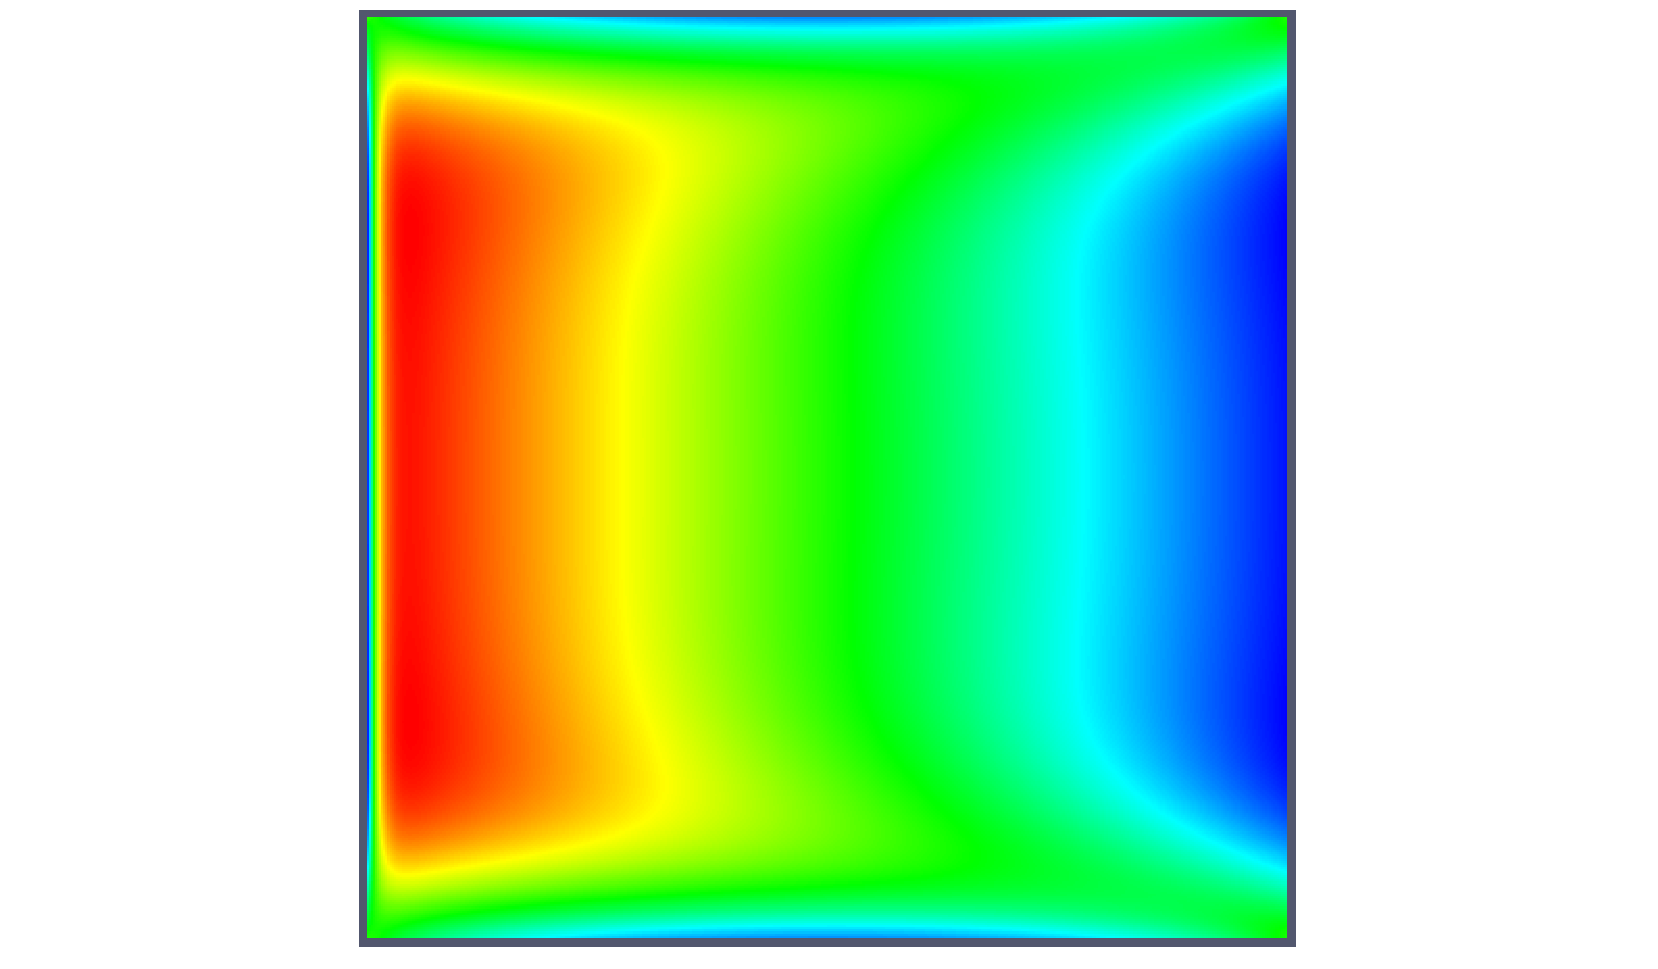
\includegraphics[width=5cm]{figs/u_graph_v_K.pdf}}
\subfigure[$\tau_x$]{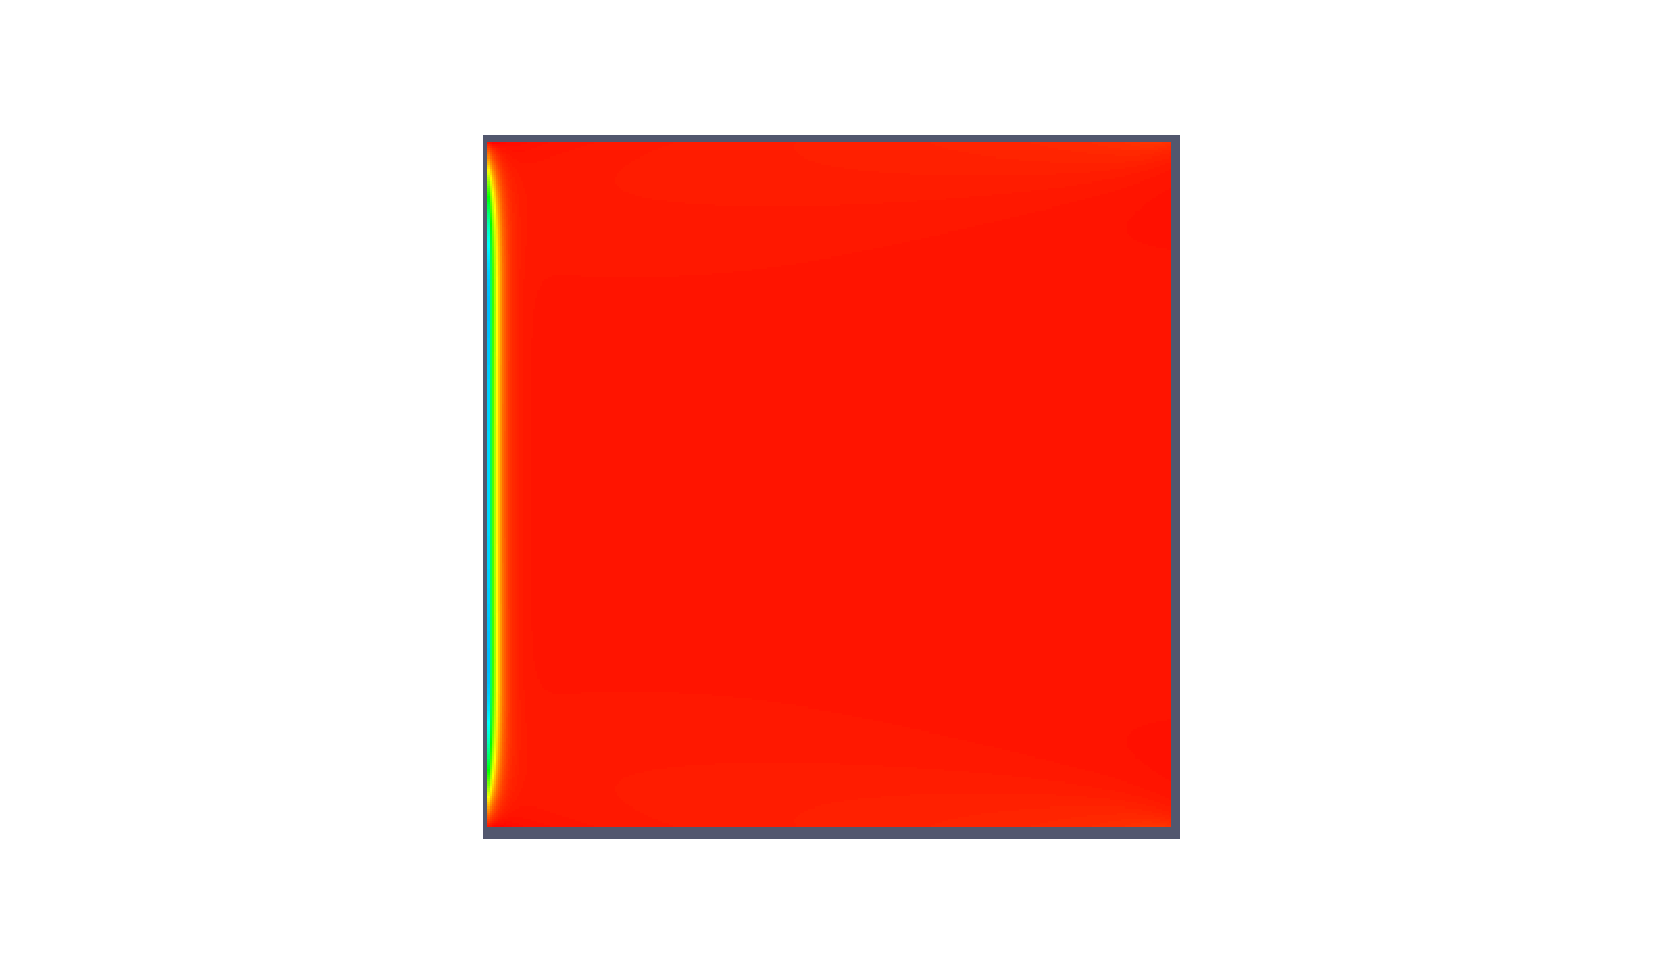
\includegraphics[width=5cm]{figs/u_graph_tau_x_K.pdf}}
\subfigure[$\tau_y$]{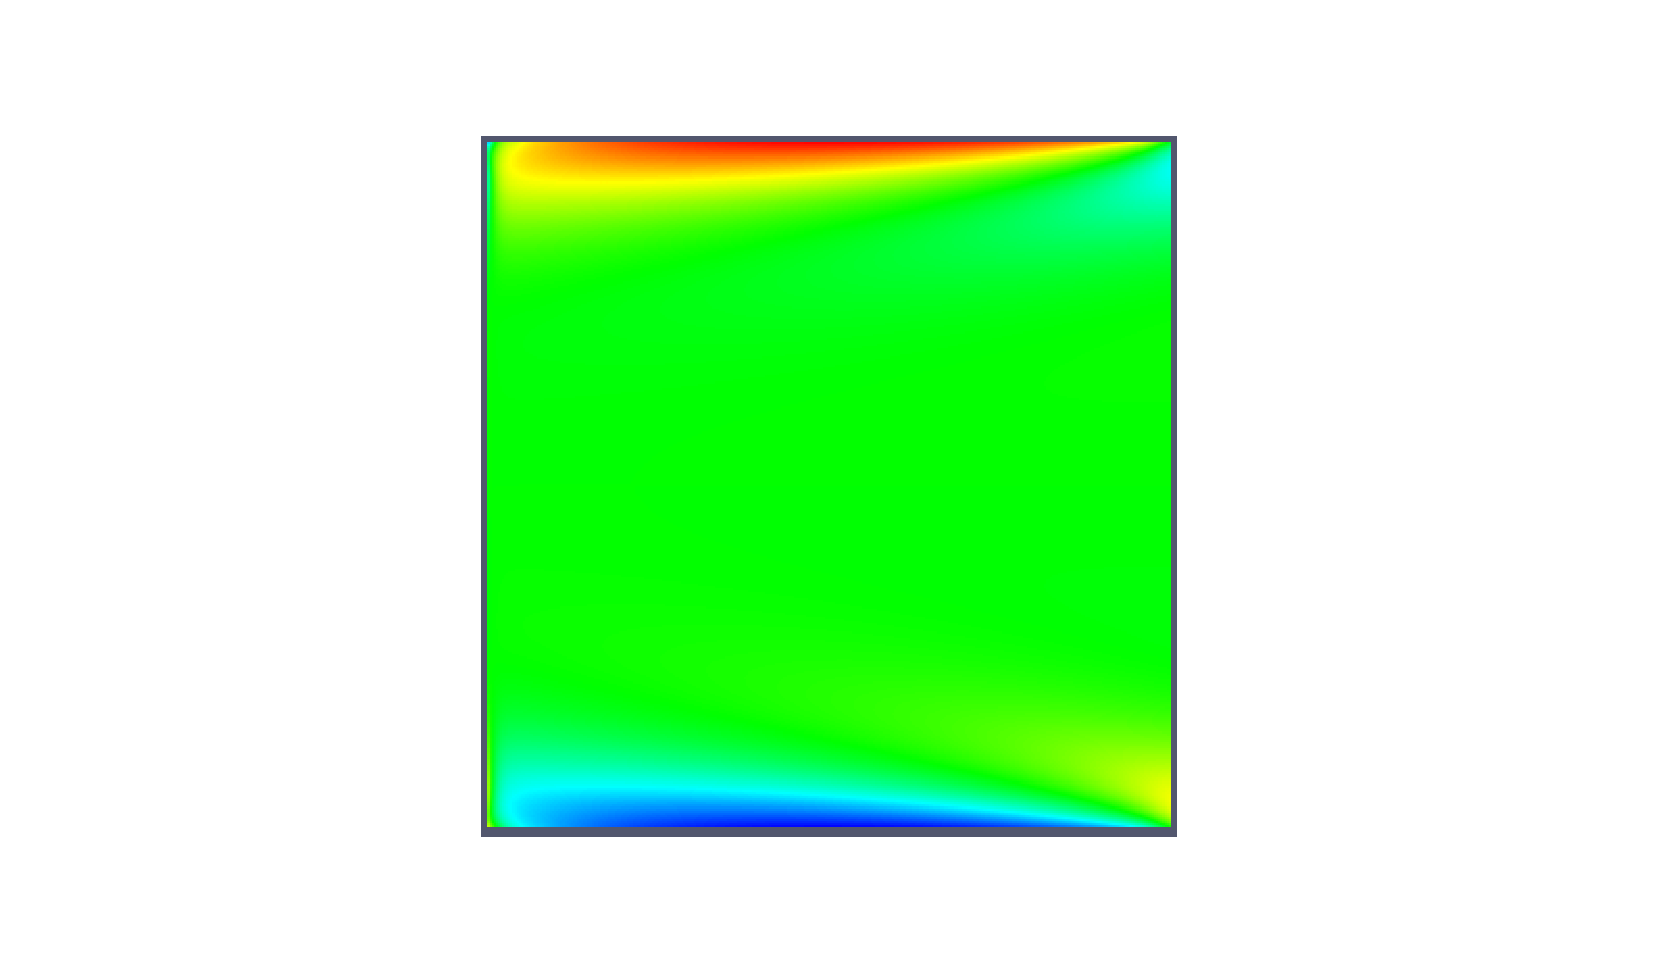
\includegraphics[width=5cm]{figs/u_graph_tau_y_K.pdf}}
\caption{$v$ and $\tau$ components of the 2D optimal test functions corresponding to the basis function $u=1$ on the reference element for $\epsilon = 0.01$. The solution has been obtained using a fine $128\times128$ mesh of triangles, with $p = 3$. }
\label{fig:optTestBoundary}
\end{figure}

Under the graph norm for convection-diffusion, Problem~(\ref{aux}) over a single element is given as
\begin{align*}
\LRp{\LRp{v,\tau},\LRp{\delta v,\delta \tau}}_{V_{\rm graph}(K)} &= \LRp{u, \Grad_h\cdot \tau - \beta\cdot \Grad_h v}_{K} + \LRp{\sigma, \frac{1}{\epsilon}\tau + \Grad_h v}_{(K)} \\
&+ \LRa{\uh,\tau_n}_{\partial K} + \LRa{\fnh,v}_{\partial K}
\end{align*}
where $\LRp{\LRp{v,\tau},\LRp{\delta v,\delta \tau}}_{V_{\rm graph}(K)}$ is 
\begin{align*}
\LRp{\LRp{v,\tau},\LRp{\delta v,\delta \tau}}_{V_{\rm graph}(K)} =& \LRp{\div\tau - \beta \cdot \grad v,\div\delta \tau - \beta \cdot \grad \delta v}_{L^2(K)} \\
&+ \LRp{{\epsilon}^{-1} \tau -  \grad v,{\epsilon}^{-1} \delta \tau -  \grad \delta v}_{L^2(K)} + \LRp{v,\delta v}_{L^2(K)} 
\end{align*}

We can transform the above problem to the reference element; applying this simple scaling argument shows that, for elements of size $h$, we can expect a boundary layer of width $h/\epsilon$ relative to a unit domain.\footnote{This is assuming that the parameter $\epsilon$ dictates the width of expected boundary layers on a unit domain. The strong form of the above variational problem corresponds to a reaction-diffusion system, for which we expect this assumption to hold.  Numerical experiments also appear to confirm that the boundary layer is of width $O(\epsilon)$.}  In other words, the strength of the boundary layer is proportional to the element Peclet number ${\rm Pe} = h/\epsilon$.  For severely underresolved meshes where $h \gg \epsilon$, this makes the approximation of optimal test functions using a simple $p$-enriched space very difficult, though specially designed $hp$-Shishkin subgrid meshes have been used to resolve such test functions with some success in \cite{DBLP:journals/procedia/NiemiCC11} (these are discussed further in Section~\ref{ShishkinSection}).  The construction of alternative test norms in \cite{DPGrobustness, ChanHeuerBui-ThanhDemkowicz12} was motivated by the computational difficulty in applying the graph test norm to heavily convection-dominated regimes where $\epsilon \ll 1$.  

Consider now globally optimal test functions under the test norm, where Problem~(\ref{aux}) is solved using the weakly conforming space $\tilde{V}$.  By the same scaling argument, strong boundary layers appear, but only at the global inflow boundary $\Gamma_{\rm in}$.  We illustrate this in Figure~\ref{fig:optTestBoundaryGlobal}, where we use an $H^1\times H({\rm div})$-conforming finite element space to approximate the globally conforming test function.  We note that, by approximating optimal test functions using a conforming test space, our test functions no longer produce boundary layers over every single element. However, in return, our optimal test functions now contain non-local information - in particular, optimal test functions for trial functions with support only in the interior of the domain now contain boundary layers at the domain inflow boundary $\Gamma_{\rm in}$.

\begin{figure}[!h]
\centering
\subfigure[$v$]{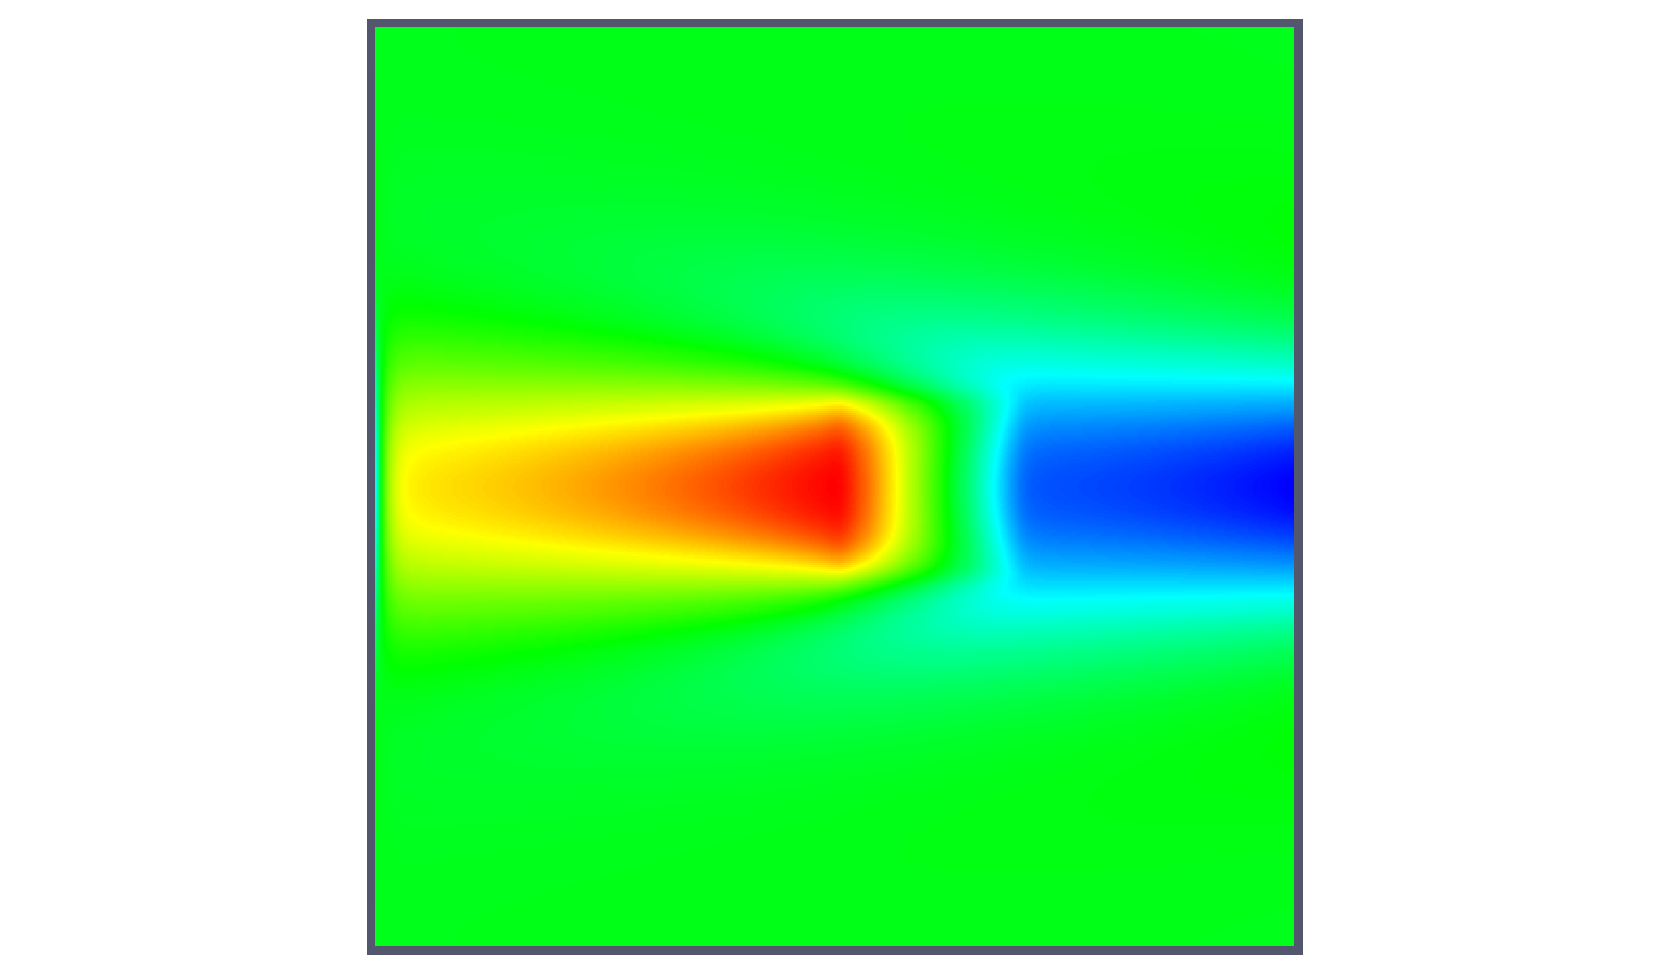
\includegraphics[width=5cm]{figs/u_graph_v.pdf}}
\subfigure[$\tau_x$]{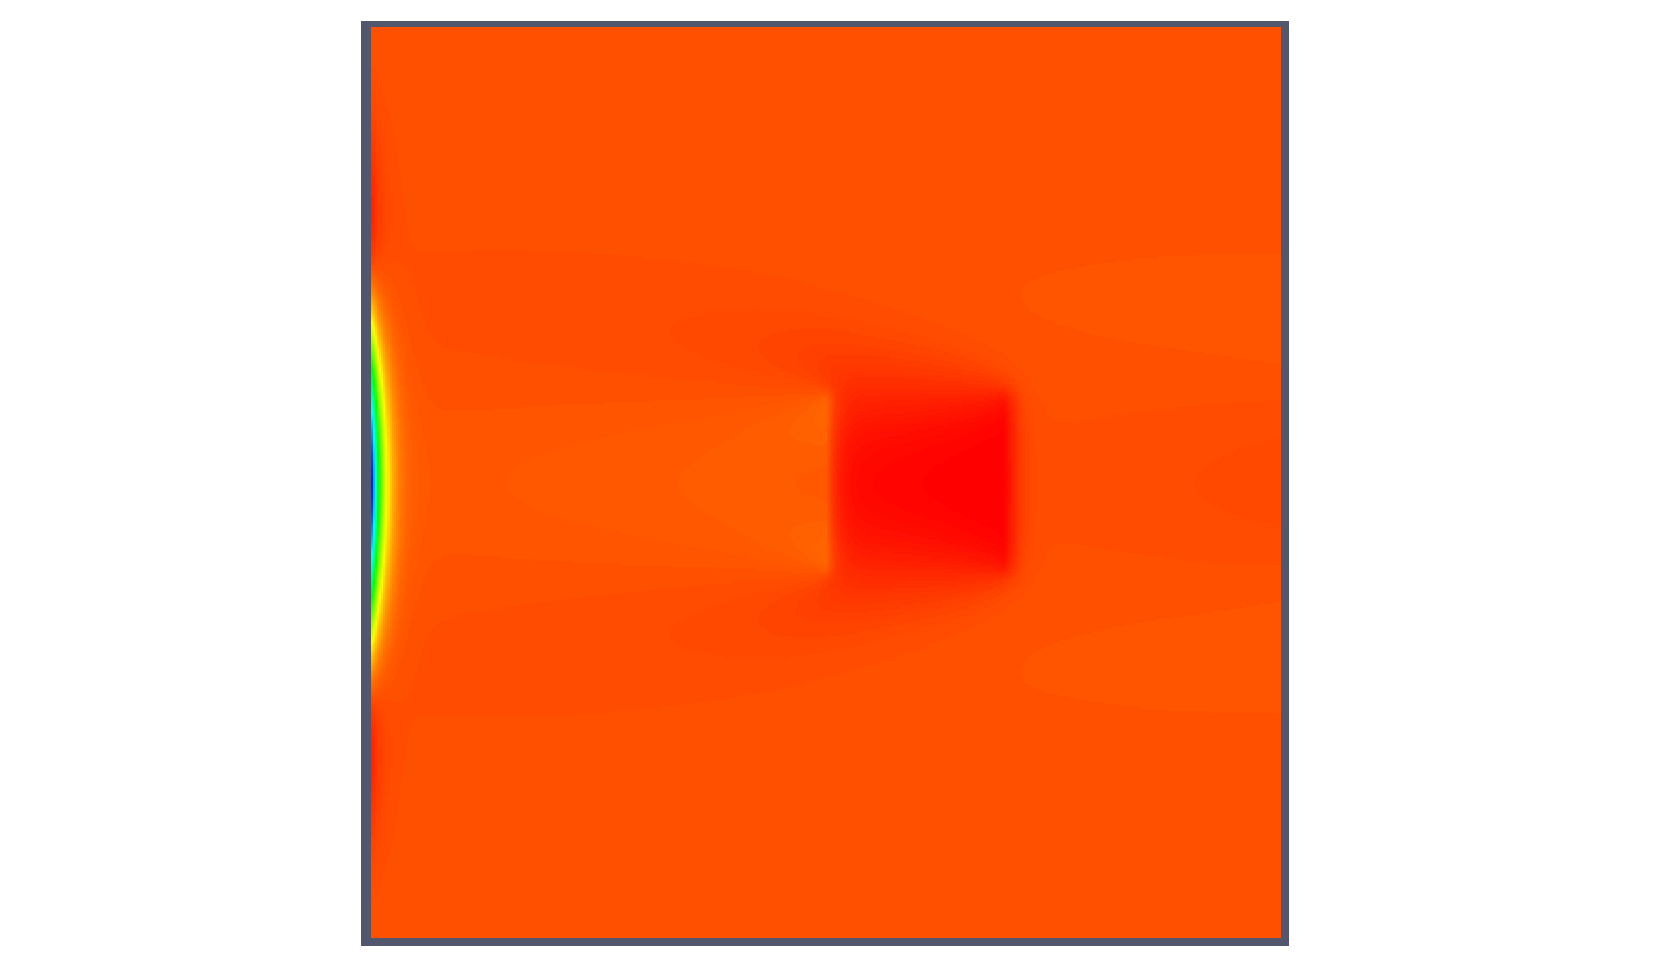
\includegraphics[width=5cm]{figs/u_graph_tau_x.pdf}}
\subfigure[$\tau_y$]{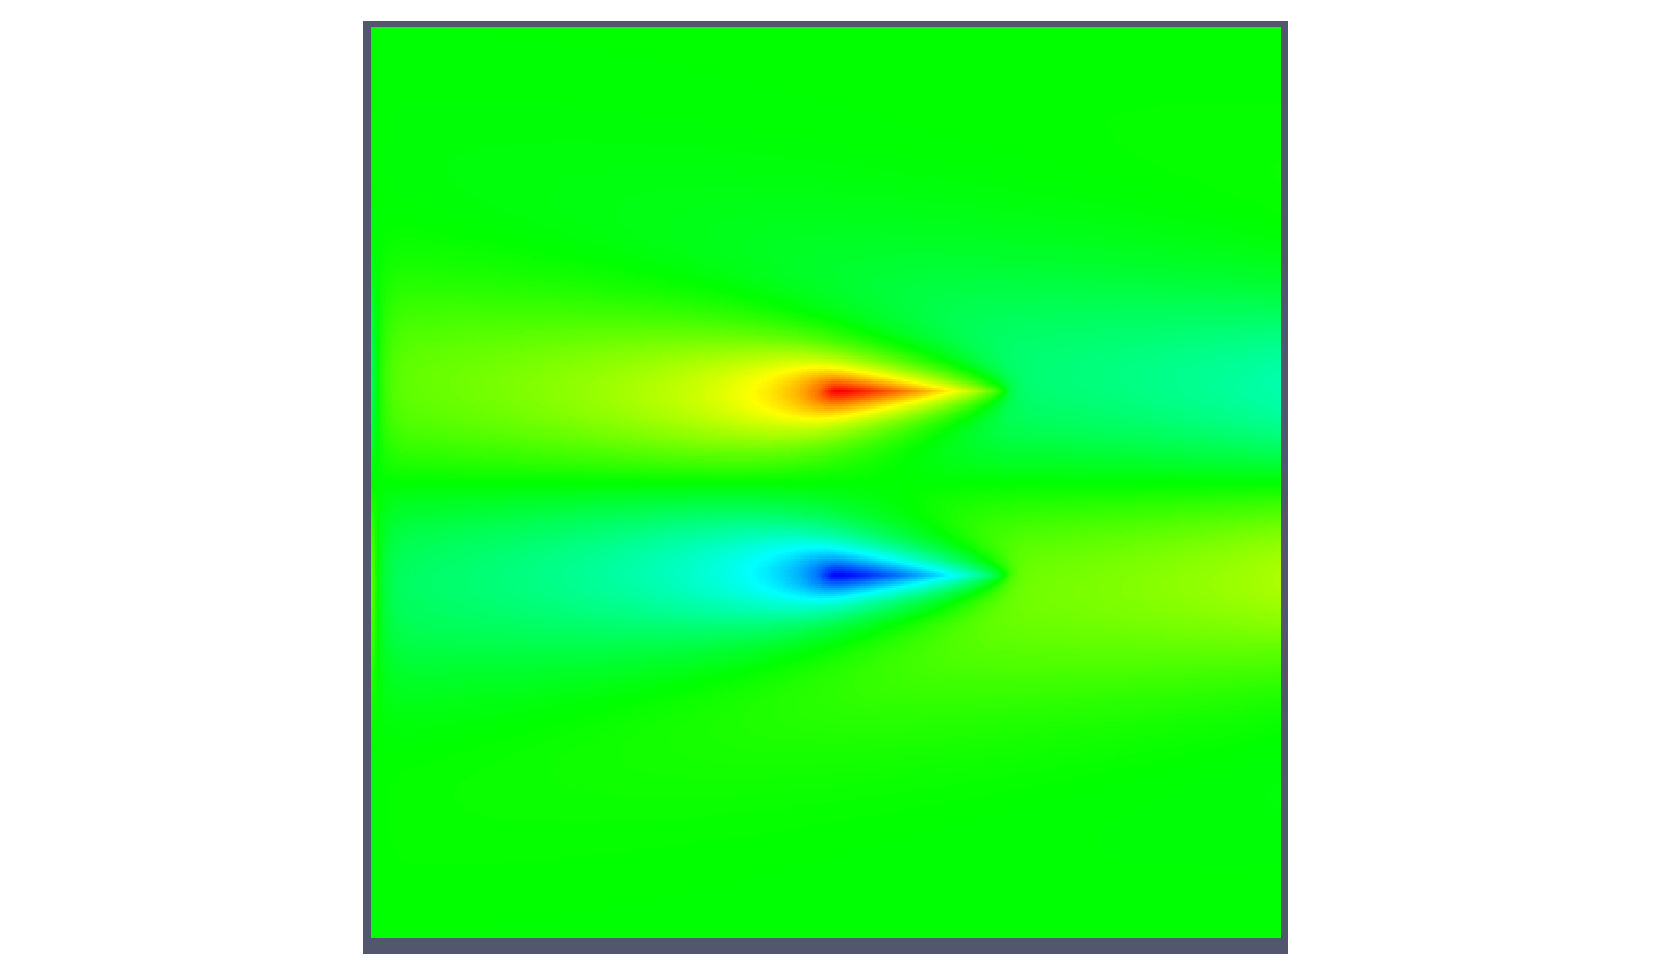
\includegraphics[width=5cm]{figs/u_graph_tau_y.pdf}}
\caption{$v$ and $\tau$ components of the 2D optimal test functions corresponding to the piecewise constant $u=1$ with support on a quad element defined on $[.5,.7]\times[.4,.6]$ for $\epsilon = 0.01$. Note the presence of nonlocal behavior in the form of the boundary layer at the inflow boundary.}
\label{fig:optTestBoundaryGlobal}
\end{figure}

In light of the non-local nature of globally optimal test functions, we might exploit the fact that, under DPG with the ultra-weak variational formulation, our locally determined test space naturally contains non-local information as well.  By Lemma~\ref{lemma1}, we know that the globally (weakly) conforming optimal test space is contained within our locally determined optimal test space; by Lemma~\ref{lemma2}, we have that the DPG solutions under local and conforming optimal test spaces coincide up to $L^2$ field variables.  In other words, the approximation of the field solution $u$ is solely determined by the approximation of globally optimal test functions by the weakly conforming space enriched space $\tilde{V}_h$.  

\section{Global effects in numerical experiments}

We investigate now non-local effects present in the DPG optimal test spaces for convection-diffusion under the test norm.  In particular, we focus on the resolution of boundary layers in optimal test functions for DPG and their effect on \textit{robustness} of discrete solutions with respect to $\epsilon$. Under fully resolved optimal test functions under the graph test norm, we expect the DPG method to be robust in $\epsilon$, and for non-robustness to be attributed to approximation error of test functions.  


\subsection{Robustness}
\label{sec:robust}
The difficulty encountered by most numerical and finite element methods for boundary layer solutions of convection-diffusion problems is a lack of \textit{robustness} in the diffusion parameter $\epsilon$; in other words, for a fixed resolution/number of degrees of freedom, as $\epsilon$ decreases, the finite element error degrades with respect to the best approximation error.  This can be seen in typical error bounds for finite element methods; if finite element error is appropriately measured in some norm $\nor{\cdot}_U$, then
\[
\frac{\nor{u-u_h}_U}{\inf_{w_h\in U_h}\nor{u-w_h}_U} = O(\epsilon^{-1}).
\]
Under naive finite elements, which relies on the coercivity of the bilinear form to provide stability, the dependence of the above ratio on $\epsilon$ can be connected to the discrete coercivity constant, which (for appropriate assumptions on boundary conditions and $\beta$) is $O(\epsilon)$ with respect to the $H^1$ norm or seminorm \cite{roos2008robust}).\footnote{These assumptions can be relaxed slightly in the presence of a first order term \cite{stynesSUPG}.}
%This degeneration of the typically manifests itself as oscillatory behavior, which can be observed in the application of the naive finite element method to the convection-dominated diffusion equation.  This issue can be slightly alleviated through the use of Shishkin meshes which anticipate the presence of boundary layers. 

\subsection{Adaptivity and adjoint boundary layers}

%\	textcolor{red}{Make note on how refinements are seen at the inflow.  Cite \cite{DPG3}, \cite{DahmenVariationalStabilization}.  Make note that the method attempts to approximate the optimal test space even when the test norm is different.}

We adopt a modification of a problem first proposed by Eriksson and Johnson in \cite{Eriksson1993} and later used in \cite{DPGrobustness, ChanHeuerBui-ThanhDemkowicz12} to determine the robustness of DPG with respect to the diffusion parameter $\epsilon$. For the choice of $\Omega = (0,1)^2$, $f=0$, and $\beta = (1,0)^T$, the convection diffusion equation reduces to
\[
\pd{u}{x} - \epsilon \left(\pdd{u}{x}+ \pdd{u}{y}\right) = 0,
\]
which has an exact solution by separation of variables, allowing us to analyze convergence of DPG for a wide range of $\epsilon$. The use of adaptive quadrature was used to ensure accurate reporting of errors for solutions with boundary layers, and all computations have been done using the higher-order adaptive DPG codebase Camellia, built on the Sandia toolbox Trilinos \cite{Camellia}.

For boundary conditions, we impose
\begin{align*}
u-\sigma_x &= u_0-\sigma_{x,0}, \quad x=0,\\
\sigma_y &=  0, \quad y=0,1,\\
u &= 0, \quad x=1.
\end{align*}
In this case, our exact solution is the series
\[
u(x,y) = C_0 + \sum_{n=1}^\infty C_n \frac{\exp(r_2(x-1)-\exp(r_1(x-1)))}{r_1\exp(-r_2) - r_2\exp(-r_1)}\cos(n\pi y),
\]
where
\begin{align*}
r_{1,2} &= \frac{1 \pm \sqrt{1 + 4 \epsilon\lambda_n}}{2 \epsilon},\\
\lambda_n &= n^2\pi^2 \epsilon.
\end{align*}
%The constants $C_n$ depend on a given inflow condition $u_0$ at $x=0$ via the formula
%\[
%C_n = \int_0^1 u_0(y) \cos(n\pi y).
%\]
%We begin with the solution taken to be the first non-constant term of the above series.  We set the inflow boundary condition to be exactly the value of $u-\sigma_x$ corresponding to the exact solution.  

\begin{figure}[h!]
\centering
\subfigure{
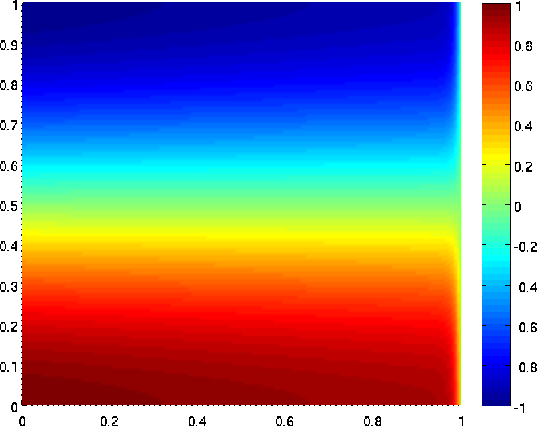
\includegraphics[scale=.37]{figs/wallBC_exact_u.png}
}
\subfigure{
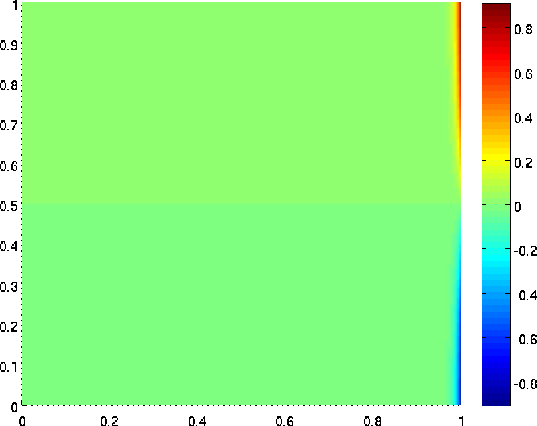
\includegraphics[scale=.37]{figs/wallBC_exact_sigx.png}
}
\subfigure{
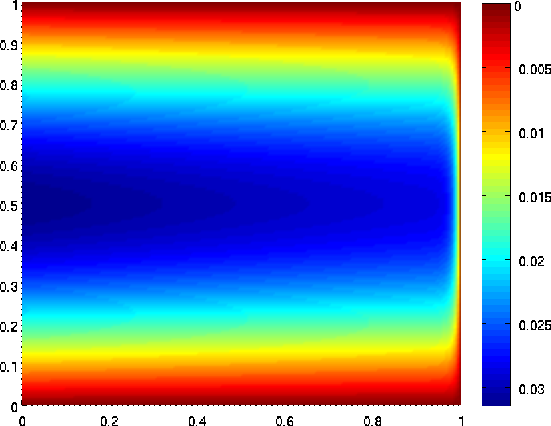
\includegraphics[scale=.37]{figs/wallBC_exact_sigy.png}
}
\caption{Exact solution for $u$, $\sigma_x$, and $\sigma_y$ for $\epsilon = .01$, $C_1 = 1$, $C_n=0$, $n\neq 1$}
\end{figure}

We begin first by recalling a phenomena observed early on in the application of DPG to convection-dominated diffusion problems.  Under the functional setting of DPG, the choice of test norm defines the optimal test space, but also defines the norm in which error is measured.  Early experiments in \cite{DPG3} by Demkowicz, Gopalakrishnan and Niemi demonstrated in computational experiments that, for naively chosen test norms, not only would the solution exhibit degeneration on a fixed mesh as $\epsilon\rightarrow 0$, but under automatic adaptivity based on the error representation function, refined meshes would tend to exhibit strong refinements at the inflow boundary.\footnote{Cohen, Dahmen and Welper reported similar results in \cite{DahmenVariationalStabilization} for a different variational formulation and test norm.  The missing factor in choosing a well-behaved test norm appears to be the presence of the $O(1)$ streamline derivative term $\nor{\beta \grad v}_{L^2}$.}  

Figure~\ref{fig:nonRobustness} shows two numerical solutions of the Erikkson-Johnson problem where the inflow profile $u_{\rm in}(y) = y(1-y)$ along $x=0$ is convected from left to right, terminating with a boundary layer at the outflow $x=1$.  The left figure shows the trial solution $u$ under a test norm introduced in \cite{DPGrobustness}, which is shown to induce a DPG method whose solutions which do not degenerate as $\epsilon\rightarrow 0$.  The presence of refinements at the inflow under the naive test norm illuminates an interesting heuristic observation concerning DPG for convection-diffusion problems; if the form of your test norm neglects to account for boundary layers in optimal test functions, their effects will show up in the energy error, and the method will still seek to resolve the optimal test space through minimization of error via adaptive mesh refinement.  

\begin{figure}[!h]
\centering
\subfigure[Robust test norm]{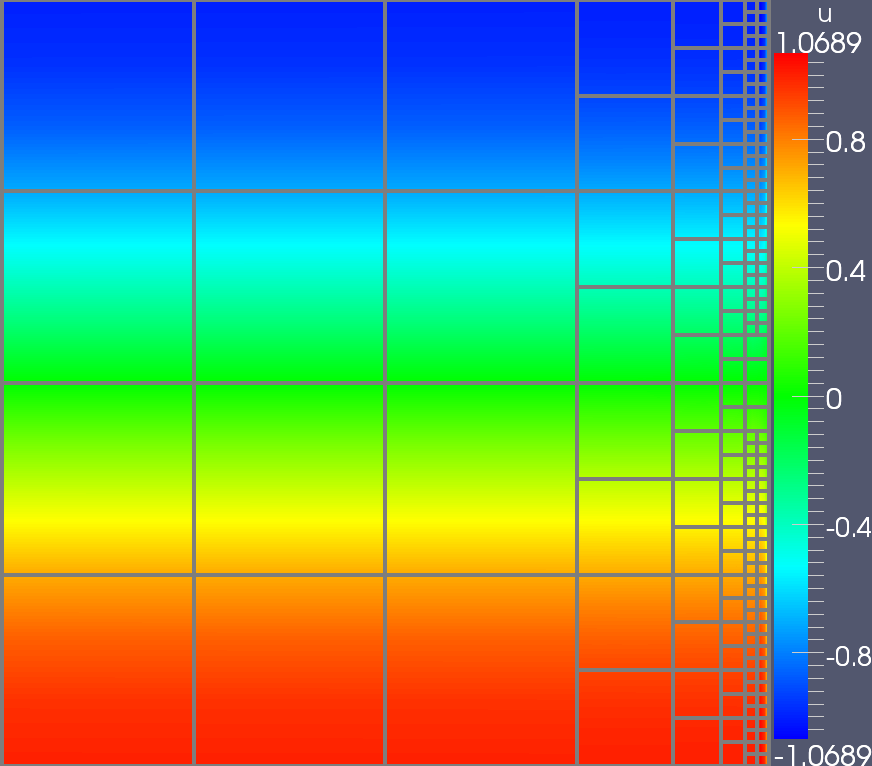
\includegraphics[width=7.5cm]{figs/robust.png}}
\subfigure[$H^1 \times H({\rm div})$ test norm]{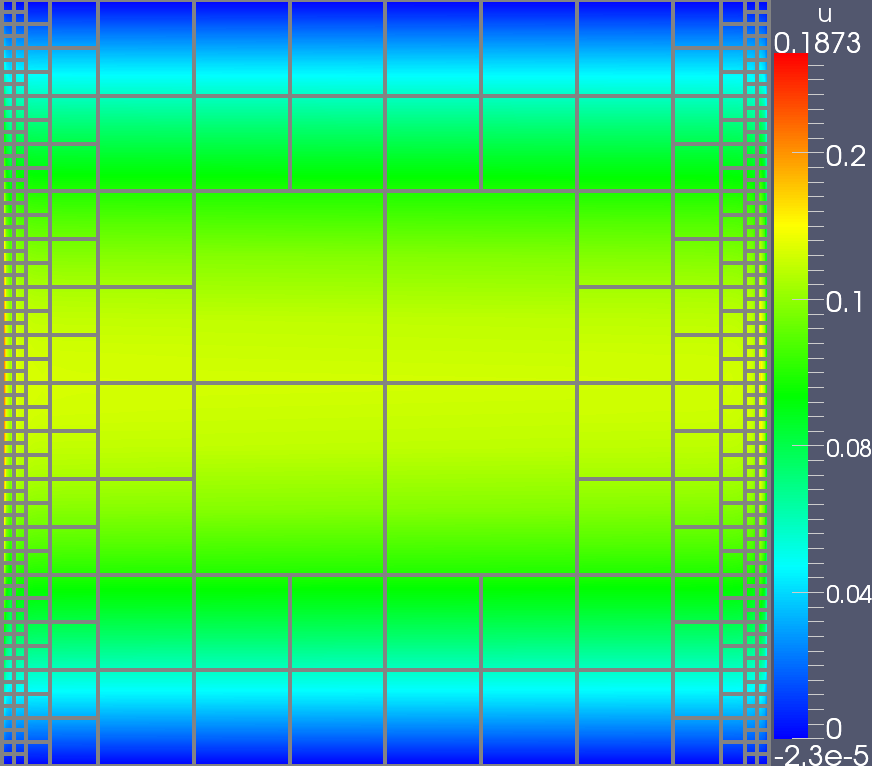
\includegraphics[width=7.5cm]{figs/nonRobust.png}}
\caption{An example of automatic mesh refinement under both a robust test norm (left) and a naively chosen non-robust test norm (right).  The naively chosen test norm exhibits both degeneration of the solution and extraneous refinements at the inflow boundary.  Both figures are produced after four automatic refinements after beginning on a uniform mesh of 4 quadratic elements with $\Delta p=3$.}
\label{fig:nonRobustness}
\end{figure}

Motivated by the phenomena observed in Figure~\ref{fig:nonRobustness}, we tested the effect of resolving the boundary layers in globally optimal test functions through the $h$-refinement of elements adjacent to the inflow boundary.  Under the graph test norm, we expect such globally determined test functions to exhibit strong boundary layers, but only at the inflow boundary.  Recalling Lemma~\ref{lemma1}, we have that the weakly conforming globally optimal test space is a proper subset of the direct sum of locally optimal test spaces over each element; thus, \textit{a-priori} refinements of the mesh that anticipate the presence of an inflow boundary layer should allow for a better resolution of the global optimal test space and improve approximation properties.  Additionally, since the solution is relatively smooth near $x=0$, we do not expect additional mesh resolution near the inflow to significantly affect the best approximation error.  

\begin{figure}[!h]
\centering
\subfigure{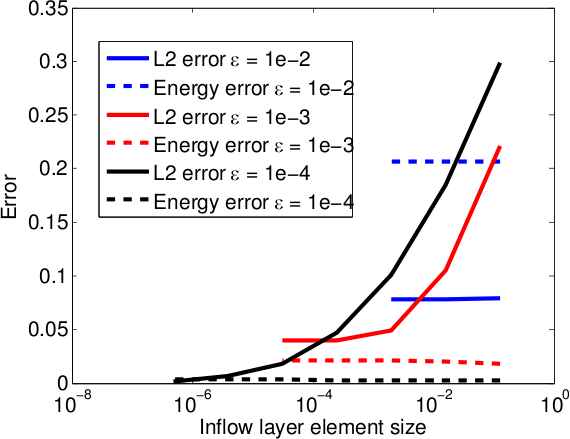
\includegraphics[width=8cm]{figs/errorInflow.png}}
\subfigure{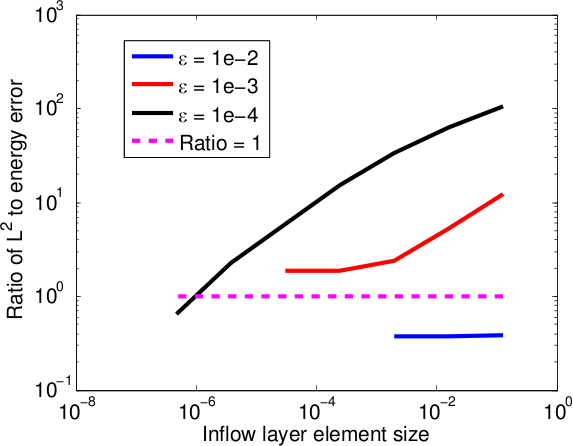
\includegraphics[width=8cm]{figs/ratioInflow.png}}
\caption{The effects of increased mesh resolution at the inflow boundary on $L^2$ and energy error (left) and their ratio (right).  Experiments were done beginning on a uniform mesh of 8-by-8 quadratic elements, with $\Delta p = 3$.}
\label{fig:robustness}
\end{figure}

Figure~\ref{fig:robustness} demonstrates the effect of increased mesh resolution at the inflow boundary; under no additional inflow resolution, the ratio of $L^2$ to energy error grows as $\epsilon$ decreases, indicating a loss of robustness as discussed in Section~\ref{sec:robust}.  However, under increased inflow resolution, the ratio can be driven down to be $O(1)$.  We expected initially for robustness to be restored under resolution of the diffusion scale; however, for $\epsilon \leq 1e-3$, achieving an $O(1)$ ratio required an order of magnitude finer resolution than the $h = O(\epsilon)$.  The reasons for this may lie in the difference between boundary layers in optimal test functions for field and flux variables and optimal test functions for trace variables.

\subsection{Under-resolution of boundary layers in optimal test functions}
\label{ShishkinSection}
We note that globally optimal test functions produce strong boundary layers at the global inflow boundary.  However, numerical experiments appear to indicate that the boundary layers in test functions for trace variables are stronger than layers in test functions for field and flux variables.  Note that the auxiliary problem for test functions under the abstract graph test norm is
\[
\LRp{v,\delta v}_{V_{\rm graph}} = \LRp{A^*_h v, A^*_h \delta v}_{L^2} + \LRp{v,\delta v}_{L^2} = \LRp{u,A^*_h v} + \LRa{\uh, v}
\]
induces a strong problem with boundary conditions $\gamma(A^*_h v) = \LRa{\uh, v}$, where $\gamma(A^*_hv)$ is the trace resulting from integration by parts of the operator $A^*_h$.  For the convection-diffusion equation, this translates to a boundary condition of 
\begin{align*}
\tau_n - \beta_n v  &= \fnh\\
\frac{1}{\epsilon}\tau_n + \pd{v}{n} &= \uh.
\end{align*}
where $\fnh$ and $\uh$ are the trace and flux variables for the convection-diffusion equation under the ultra-weak variational formulation.  The presence of the $\frac{1}{\epsilon}$ term in the boundary condition further increases the strength of the boundary layer when the auxiliary problem~(\ref{aux}) is loaded with a non-zero $\uh$.  

Figure~\ref{fig:bl_underresolution} shows the magnitude of the $\tau$ component of optimal test functions for a trace loaded on the inflow boundary for quadratic meshes with increasing anisotropic resolution in the $x$-direction.  Even between the over-resolved cases $h_x \approx \epsilon$, $h_x \approx 2^{-1}\epsilon$, and $h_x \approx 2^{-2}\epsilon$, the observed boundary layer in the optimal test functions continues to grow in magnitude (as evidenced by Table~\ref{table:magnitudes}, implying that mesh resolution at the diffusion scale is still insufficient to resolve these features.  

\begin{figure}[!h]
\centering
\subfigure[$128\times 128$ mesh]{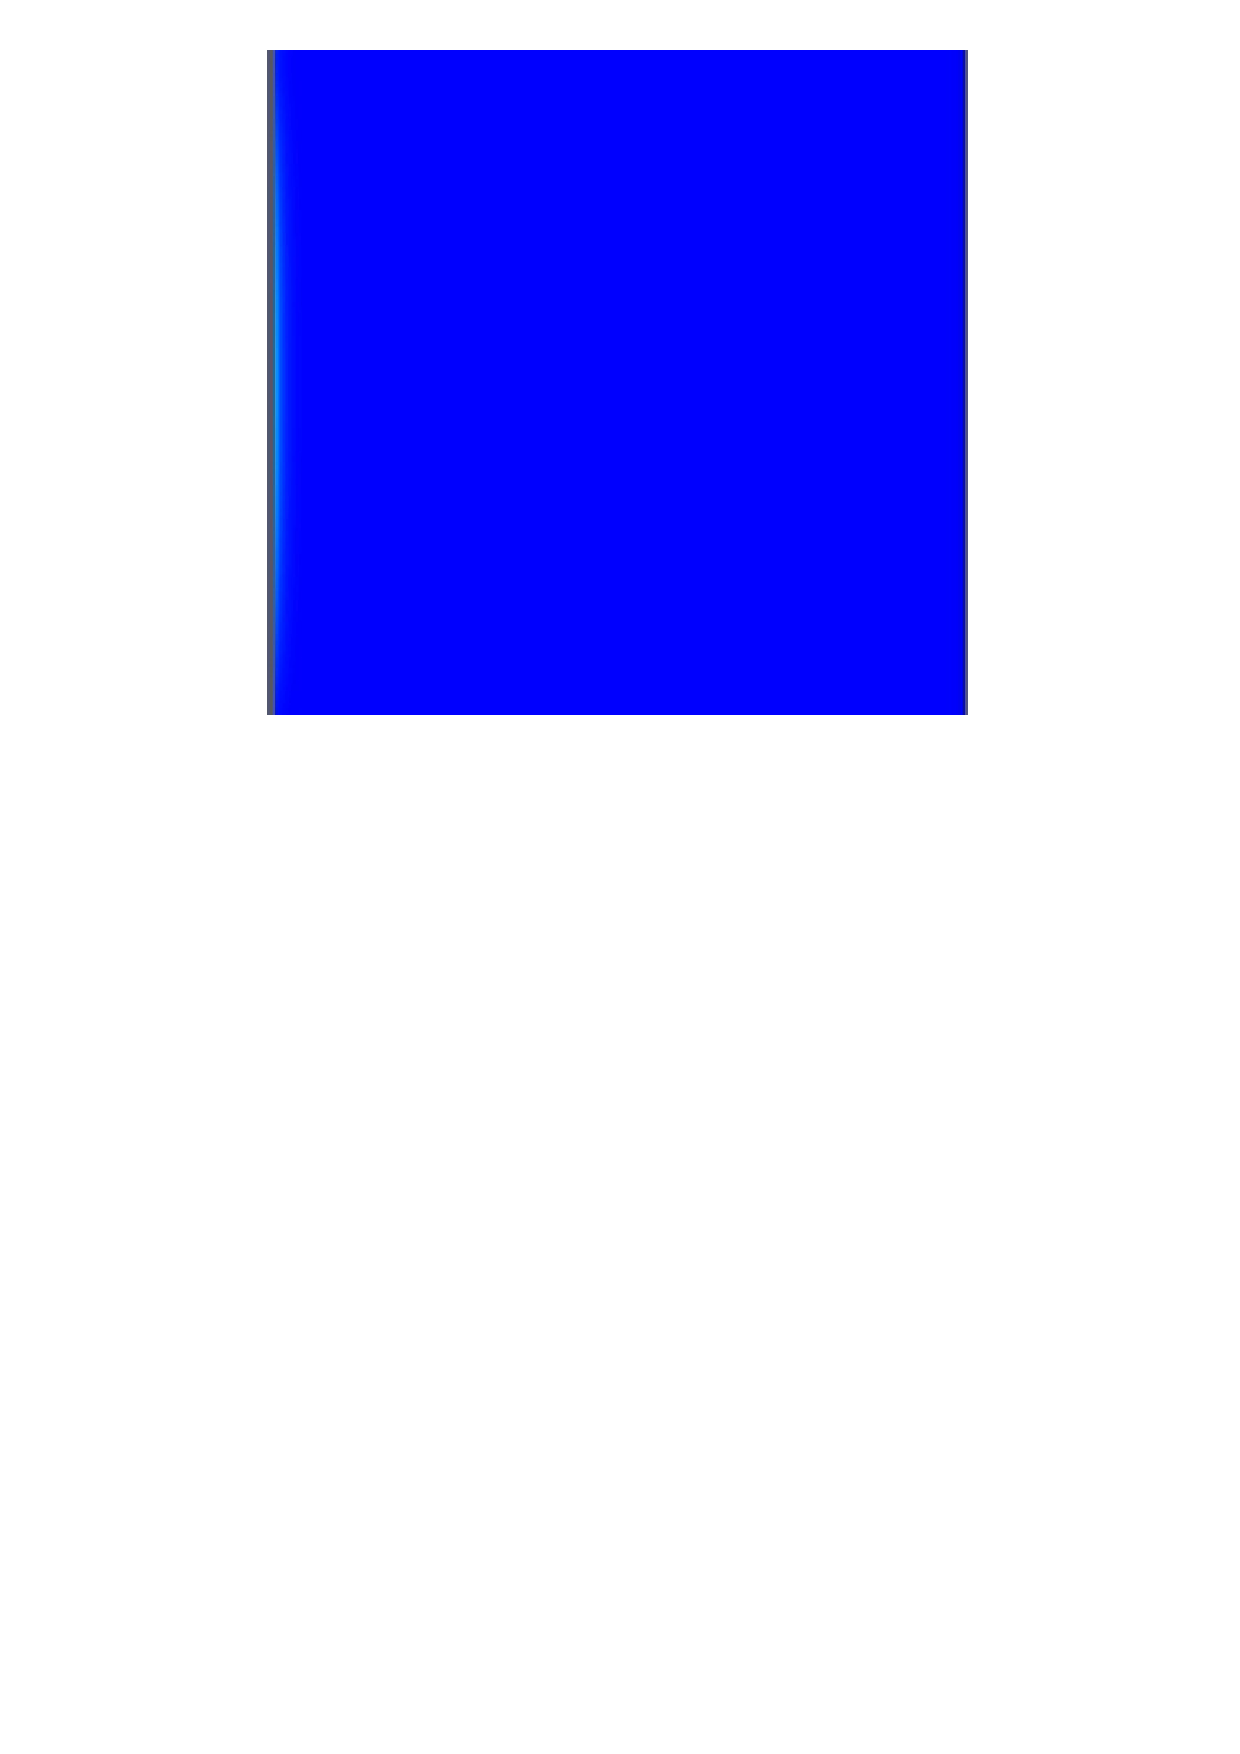
\includegraphics[height=4.7cm]{figs/uhat_graph_tau_128.pdf}}
\subfigure[$256 \times 128$ mesh]{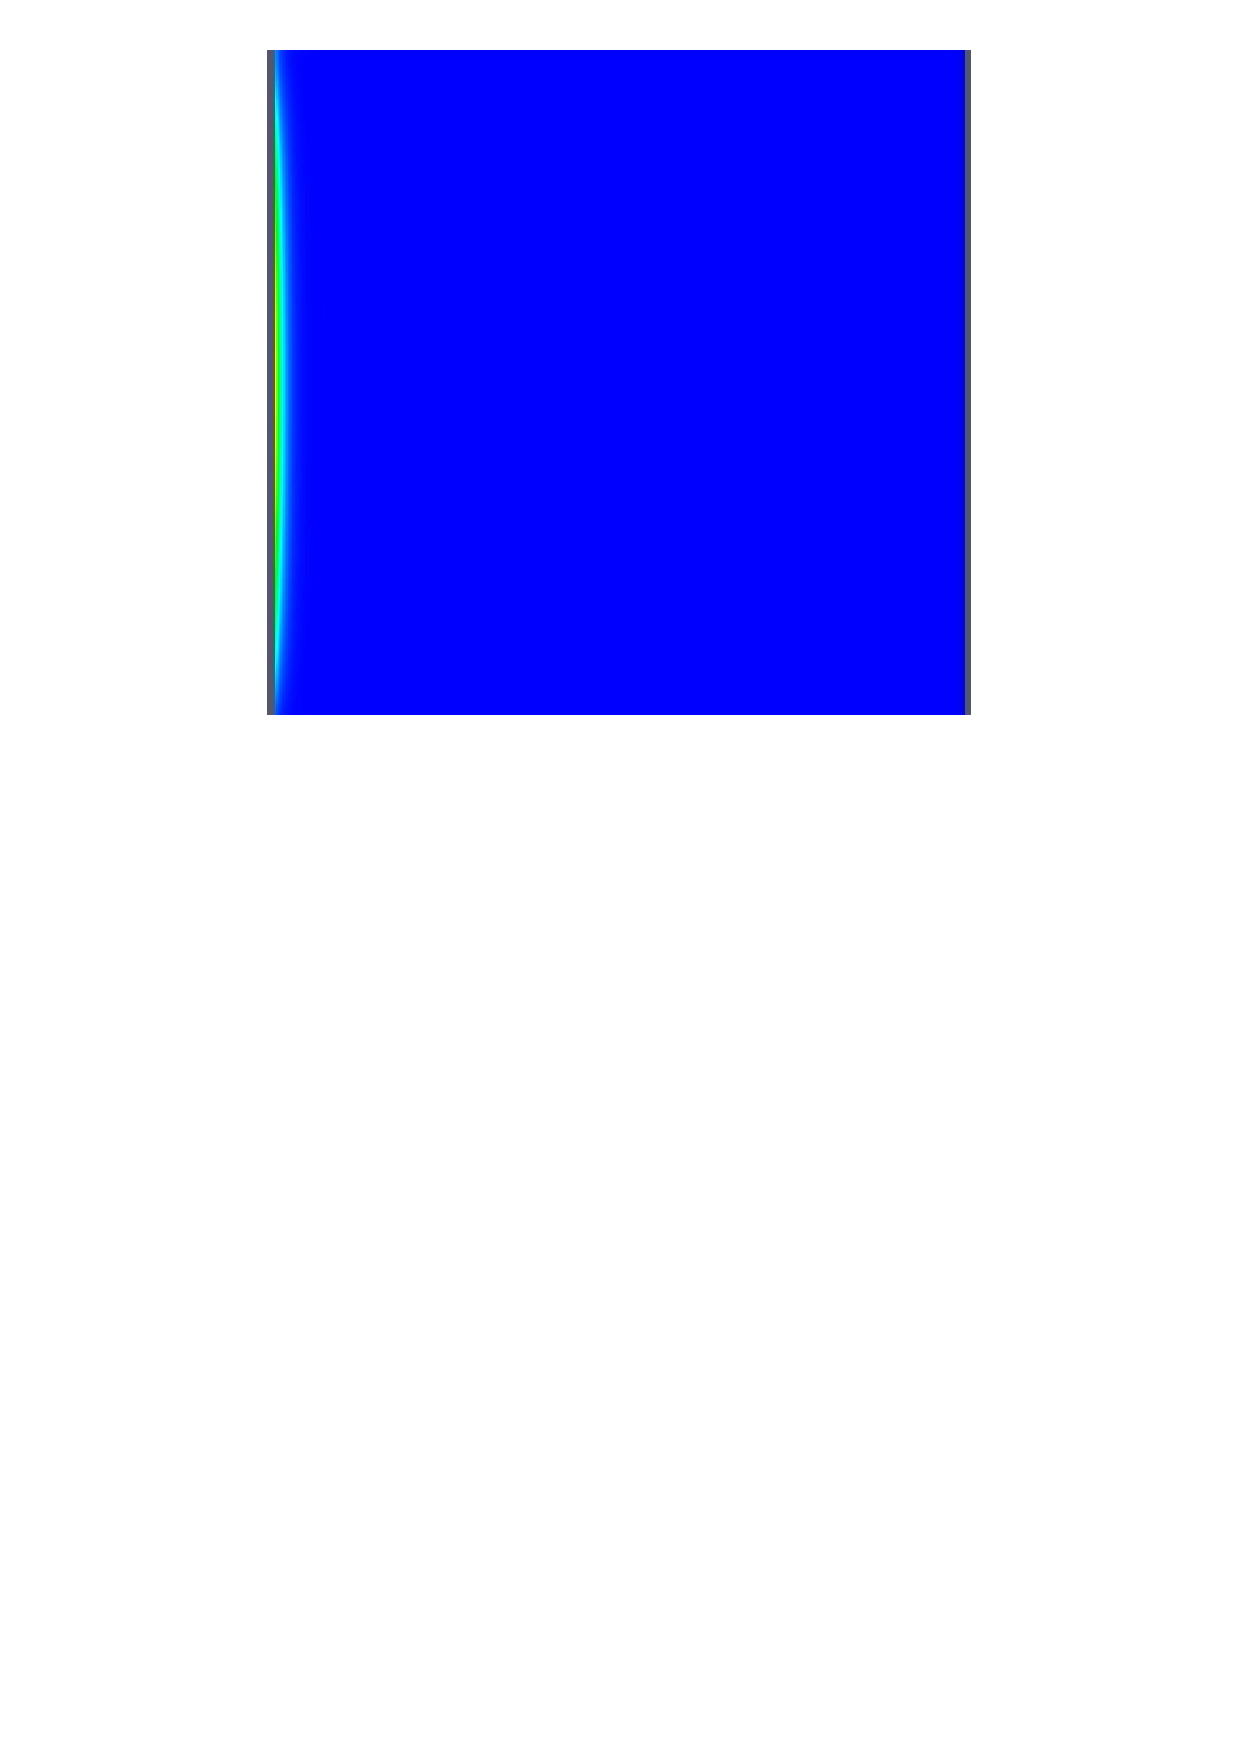
\includegraphics[height=4.7cm]{figs/uhat_graph_tau_256.pdf}}
\subfigure[$512\times 128$ mesh]{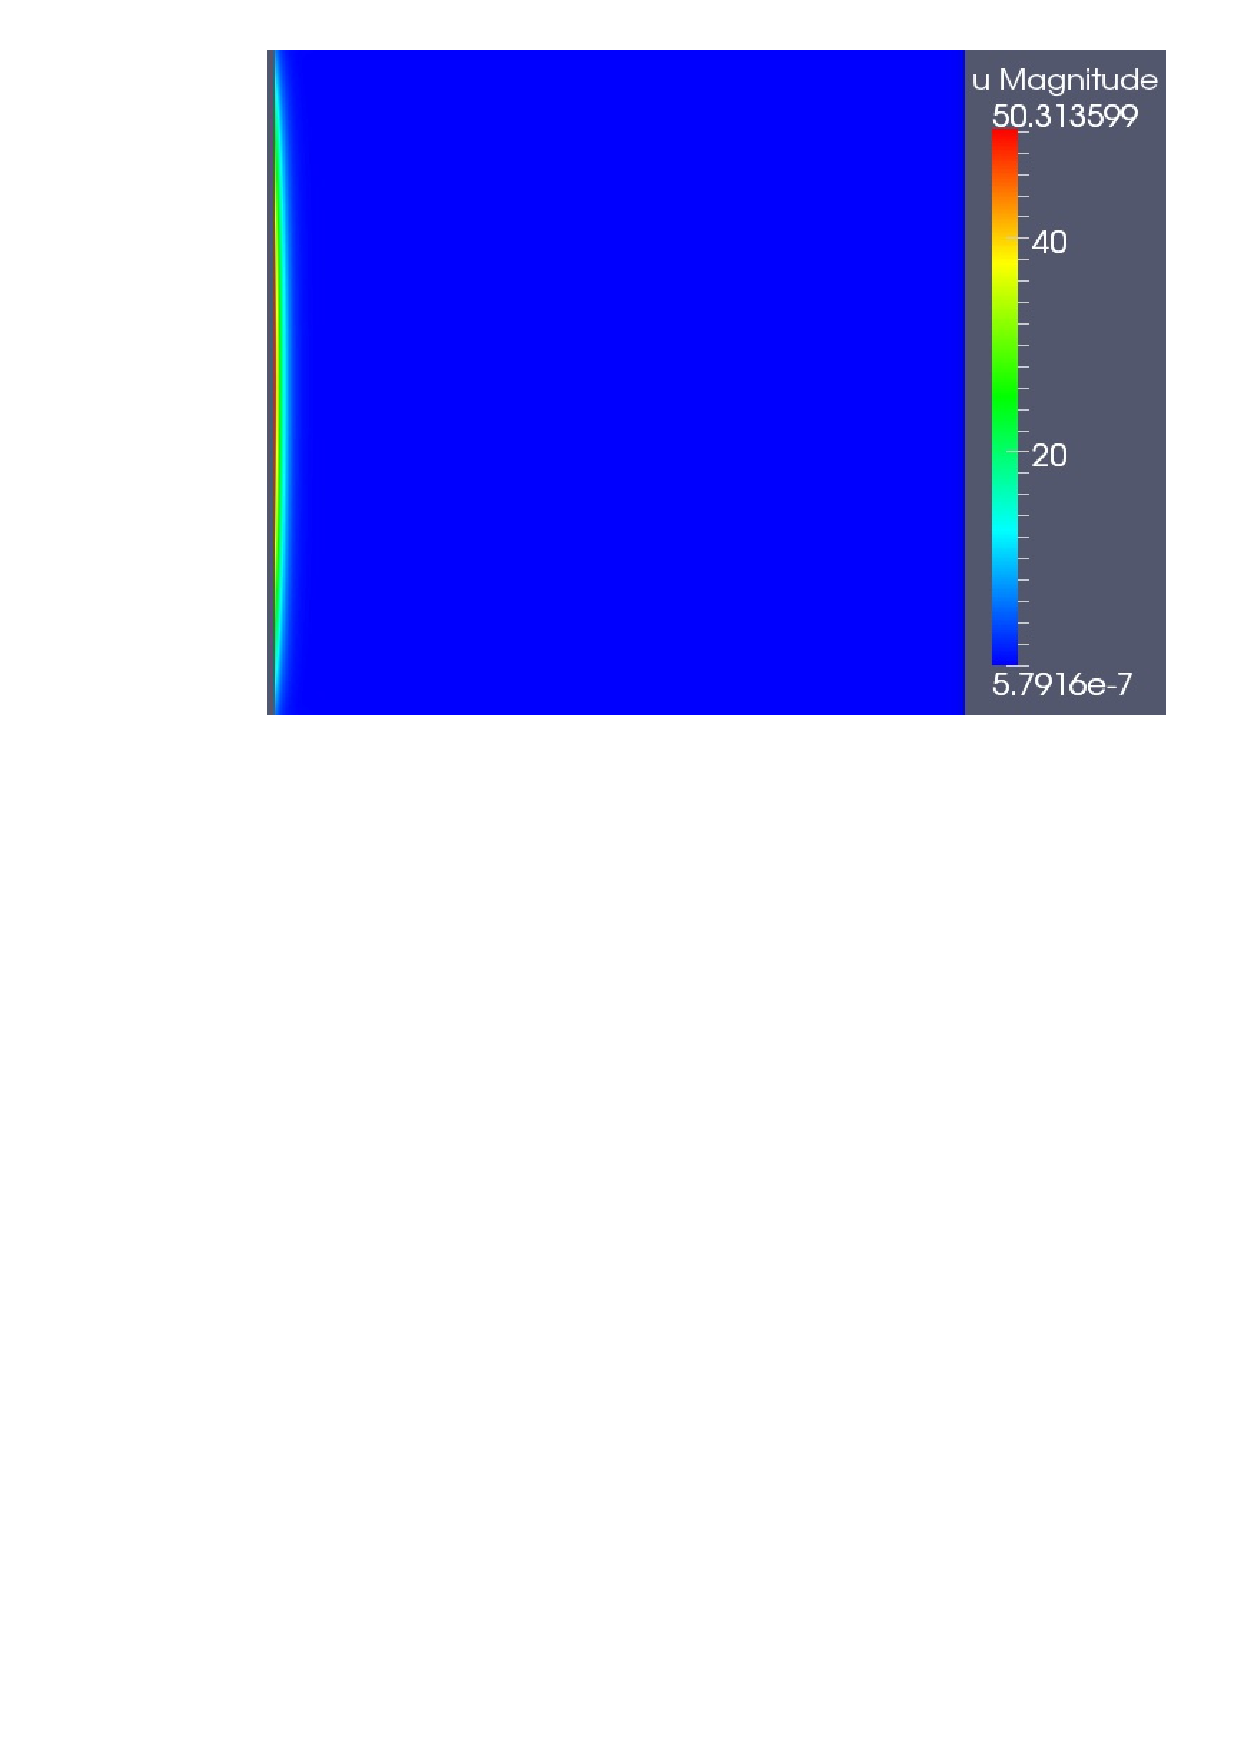
\includegraphics[height=4.7cm]{figs/uhat_graph_tau_512.pdf}}
\caption{Magnitudes of the vector-valued component $\tau$ of the optimal test functions corresponding to the flux $\widehat{u}=y(1-y)$ on the boundary $x = 0$ for $\epsilon = 0.01$ over the reference element.  }
\label{fig:bl_underresolution}
\end{figure}

This phenomena was observed also in \cite{shishkinDPG}, where $hp$-Shishkin submeshes (discussed in \cite{SchwabBoundaryLayers}) were used to resolve optimal test functions locally over an element.  In 1D, these meshes consist of a two small ``needle" elements of size $h=p \epsilon$, where $p$ is the polynomial order of the approximating functions (the 2D extension for quadrilateral elements in 2D is straightforward, and is given in detail in \cite{shishkinDPG}).  Experiments using $p$-refined Shishkin subgrid meshes indicated that the relative error in the approximation of optimal test functions for traces $\uh$ on the inflow boundary did not converge to zero as the dimension of the enriched space $V_h$ was increased (unlike the relative error for optimal test functions for field variables $u$, $\sigma$, and flux $\fnh$), and it was concluded that the use of Shishkin meshes was insufficient to resolve the boundary layers present in optimal test functions for traces over inflow edges for sufficiently small $\epsilon$.

\begin{table}
  \label{table:magnitudes}
  \begin{center}
  \begin{tabular}{|| l || c || r   }
    \hline
    Mesh & Maximum value of $| \tau_{\uh} |$ for $\epsilon=.01$ \\ \hline
    $128\times 128$ & 8.6510571  \\ \hline
    $256\times 128$ & 38.794881  \\ \hline
    $512\times 128$ & 50.313599  \\
    \hline
  \end{tabular}
\end{center}
\caption{Maximum magnitudes of the $\tau$ component of the optimal test functions corresponding to the flux $\widehat{u}=y(1-y)$ on the boundary $x = 0$ for $\epsilon = 0.01$ over the reference element.  }
\end{table}

The result of this under-resolution of optimal test functions having to do with traces on the inflow boundary is an underestimation of the inflow boundary term $\LRa{\uh,\jump{v}}_{\Gamma_{\rm in}}$, which leads to the underestimation of the solution in experiments \cite{shishkinDPG}, and explains the fine mesh resolution on the inflow boundary necessary to restore robustness to the DPG method in Figure~\ref{fig:robustness}.  

\section{Conclusions}

In this paper, we show how DPG's locally constructed test space can be interpreted as a non-conforming approximation of a weakly-conforming global test space.  Furthermore, the field solutions and trace solutions on the boundary $\Gamma$ are shown to depend \textit{only} upon properties of the non-conforming global test space; thus, when considering approximation error in test functions, resolution of global approximation error (as opposed to local approximation error) can be sufficient to produce a stable method.

Additionally, global properties of test spaces are given under which the ultra-weak formulation delivers the best $L^2$-approximation to the exact solution.  A connection is made to DPG through the graph test norm, which can be viewed as a regularization of the graph seminorm through the addition of an $L^2$ term of magnitude $\delta$. As the regularization parameter $\delta \rightarrow 0$, DPG under this version of the graph test norm is shown to converge to a weakly-conforming approximation to the $L^2$-optimal test space.  

Finally, viewing DPG as an approximation to globally optimal test functions allows the construction of test spaces that focus on resolution of global features as opposed to local features.  We illustrate this with the convection-diffusion problem, where we show that it is possible to restore robustness with respect to the diffusion parameter $\epsilon$ by neglecting the resolution of boundary layers on the element-local level and focusing on the resolution of global boundary layers in optimal test spaces.  

%\section{Acknowledgements}
%
%The authors thanks John Evans for several helpful discussions on the ideas and philosophy behind Variational Multiscale finite element methods.  

\bibliographystyle{plain}
\bibliography{paper}


\end{document}

%\subsection{The strong form of the trial-to-test operator}
%
%Under the graph test norm 
%\[
%\LRp{v,\delta v}_{V(K)} = \LRp{A_h^*v,A_h^*\delta v}_{L^2(K)} + (v,\delta v)_{L^2(K)},
%\]
%element-local test functions are induced as solutions of 
%\[
%\LRp{v,\delta v}_{V(K)} = (u,A_h^*\delta v)_K + \LRa{\uh,\delta v}_{\partial K}
%\]
%Under proper regularity assumptions, this variational problem corresponds to the strong problem
%\begin{align*}
%A_hA_h^*v + v &= A_hu, \quad \text{on $K$}\\
%\gamma\LRp{A_h^*v} &= \uh.
%\end{align*}
